%
% $RCSfile: statics_and_dynamics.tex,v $
%
% Copyright (C) 2002-2008. Christian Heller.
%
% Permission is granted to copy, distribute and/or modify this document
% under the terms of the GNU Free Documentation License, Version 1.1 or
% any later version published by the Free Software Foundation; with no
% Invariant Sections, with no Front-Cover Texts and with no Back-Cover
% Texts. A copy of the license is included in the section entitled
% "GNU Free Documentation License".
%
% http://www.cybop.net
% - Cybernetics Oriented Programming -
%
% http://www.resmedicinae.org
% - Information in Medicine -
%
% Version: $Revision: 1.1 $ $Date: 2008-08-19 20:41:09 $ $Author: christian $
% Authors: Christian Heller <christian.heller@tuxtax.de>
%

\chapter{Statics and Dynamics}
\label{statics_and_dynamics_heading}
\index{Statics and Dynamics}
\index{Static Knowledge}
\index{Dynamic Processing}

\begin{flushright}
    \textsl{I think therefore I am.}\\
    \textsc{Rene Descartes}
\end{flushright}

\begin{wrapfigure}[5]{r}{4cm}
    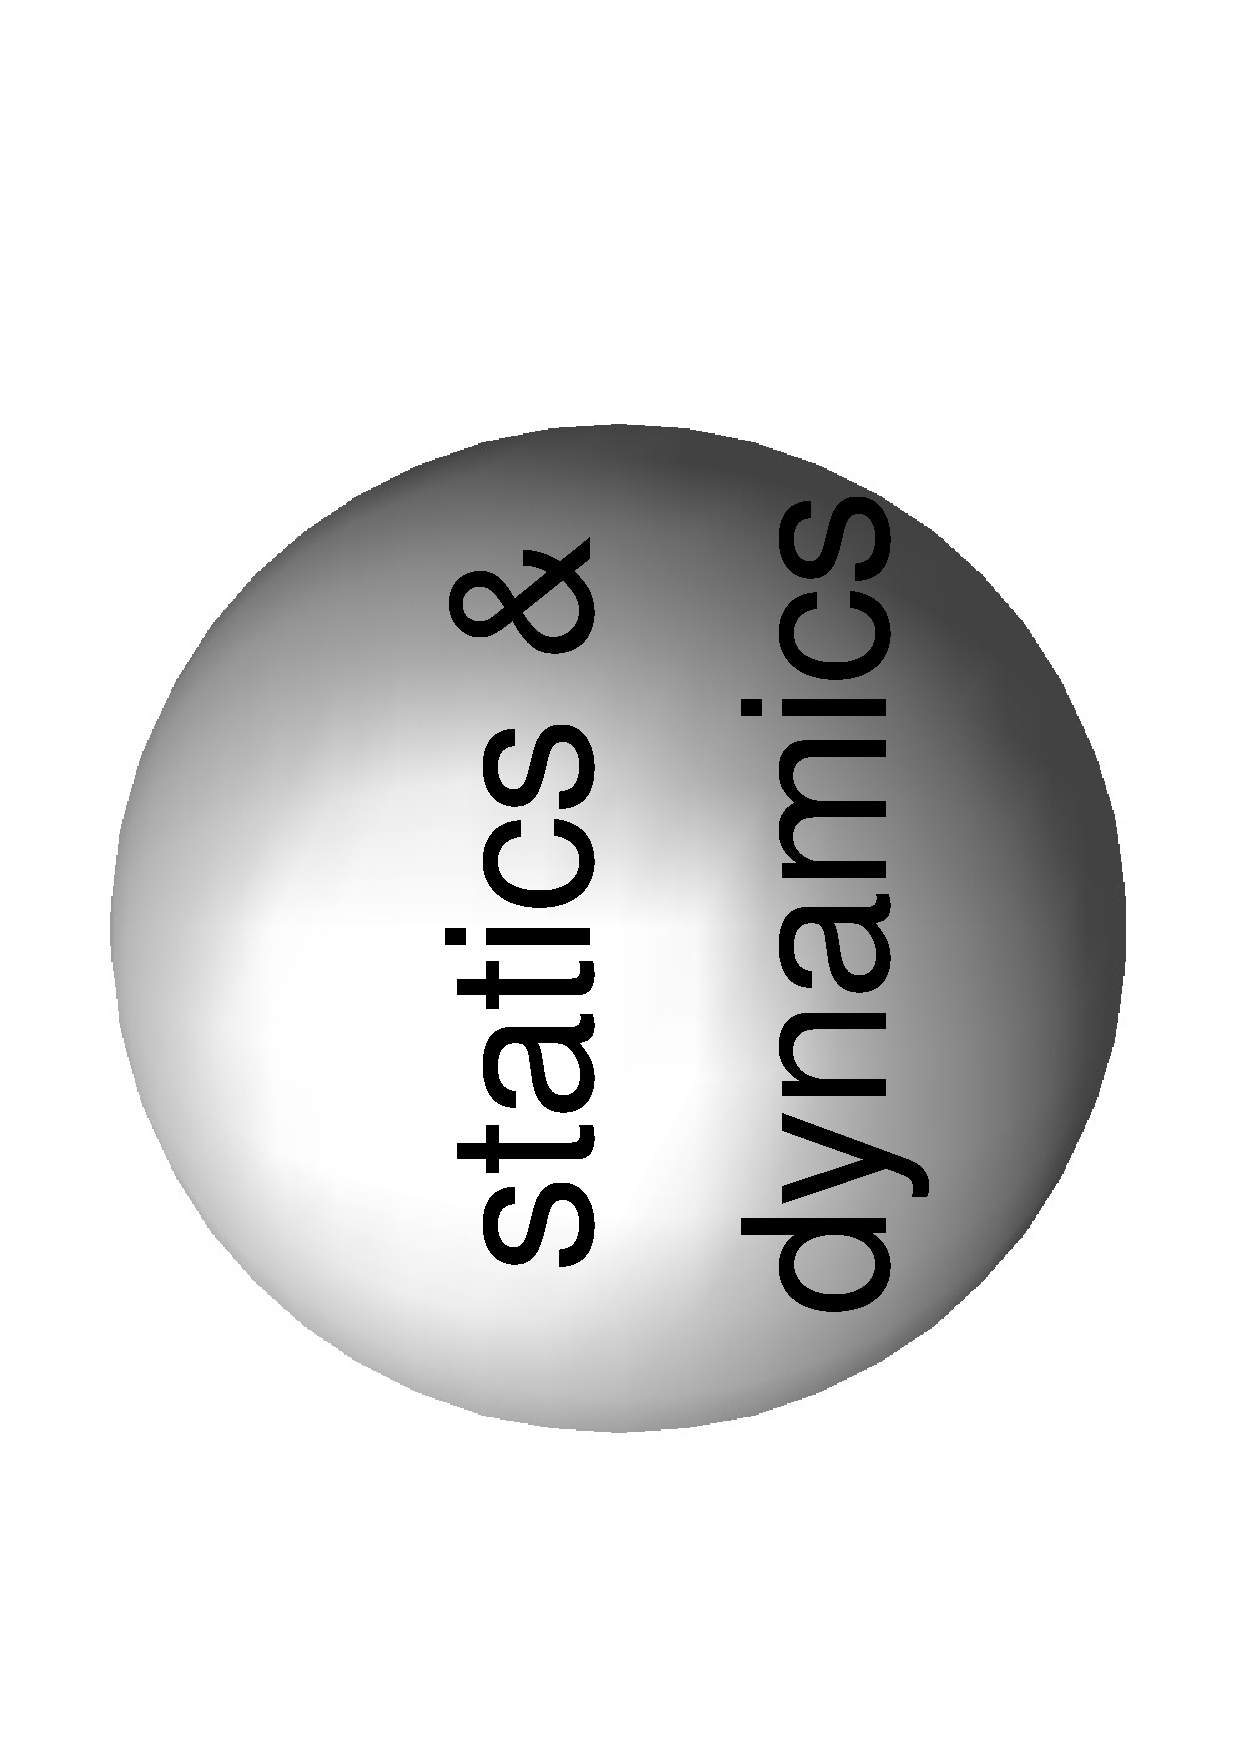
\includegraphics[scale=0.15,angle=-90]{graphic/contribution1.pdf}
\end{wrapfigure}

As first of the three main topics of part \ref{contribution_heading} of this
work, this chapter investigates how a separation of \emph{Static Knowledge}
from its \emph{Dynamic Processing} in a system can be justified. The later
chapters \ref{knowledge_schema_heading} and \ref{state_and_logic_heading} will
deal with the structuring of knowledge.
\vspace{1cm}

%
% $RCSfile: virtual_and_real_world.tex,v $
%
% Copyright (C) 2002-2008. Christian Heller.
%
% Permission is granted to copy, distribute and/or modify this document
% under the terms of the GNU Free Documentation License, Version 1.1 or
% any later version published by the Free Software Foundation; with no
% Invariant Sections, with no Front-Cover Texts and with no Back-Cover
% Texts. A copy of the license is included in the section entitled
% "GNU Free Documentation License".
%
% http://www.cybop.net
% - Cybernetics Oriented Programming -
%
% http://www.resmedicinae.org
% - Information in Medicine -
%
% Version: $Revision: 1.1 $ $Date: 2008-08-19 20:41:09 $ $Author: christian $
% Authors: Christian Heller <christian.heller@tuxtax.de>
%

\section{Virtual- and Real World}
\label{virtual_and_real_world_heading}
\index{Virtual- and Real World}

A separate treatment of knowledge and system functionality can be observed in
many fields of science. Some examples are given following.

%
% $RCSfile: mind_and_body.tex,v $
%
% Copyright (C) 2002-2008. Christian Heller.
%
% Permission is granted to copy, distribute and/or modify this document
% under the terms of the GNU Free Documentation License, Version 1.1 or
% any later version published by the Free Software Foundation; with no
% Invariant Sections, with no Front-Cover Texts and with no Back-Cover
% Texts. A copy of the license is included in the section entitled
% "GNU Free Documentation License".
%
% http://www.cybop.net
% - Cybernetics Oriented Programming -
%
% http://www.resmedicinae.org
% - Information in Medicine -
%
% Version: $Revision: 1.1 $ $Date: 2008-08-19 20:41:07 $ $Author: christian $
% Authors: Christian Heller <christian.heller@tuxtax.de>
%

\subsection{Mind and Body}
\label{mind_and_body_heading}
\index{Mind and Body}
\index{Philosophy}
\index{Metaphysics}
\index{Ontology}
\index{Knowledge}
\index{Dualism}
\index{Being}
\index{Hardware}
\index{Software}
\index{Operating System}
\index{OS}

In \emph{Philosophy}, it is common to distinguish between two traditions:
Euro-American \emph{Western Philosophy} and Asian \emph{Eastern Philosophy}
\cite{wikipedia}. The former, also called \emph{Western Academic Philosophy},
is often divided into: \emph{Analytic-} and \emph{Continental Philosophy}.
While continental philosophy is predominant in continental Europe, analytic
philosophy dominates Anglo-American philosophy. Western philosophy has its
roots in ancient \emph{Greek Philosophy}, which, among others, dealt with five
broad types of analytical questions \cite{wikipedia}:

\begin{itemize}
    \item[-] \emph{metaphysical:} study of any of the most fundamental concepts
        and beliefs about the basic nature of \emph{Reality}, such as
        \emph{Ontology} as the science of \emph{Being}
    \item[-] \emph{epistemological:} study of the nature, origin and scope of
        \emph{Knowledge}
    \item[-] \emph{logical:} study of \emph{Inference}, that is \emph{Reasoning}
        used to reach a conclusion from a set of assumptions
    \item[-] \emph{ethical:} study of \emph{Morality}, that is behaviour which
        is \emph{good}
    \item[-] \emph{aesthetic:} study of the nature of \emph{Beauty}
\end{itemize}

To the metaphysical questions belong:

\begin{itemize}
    \item[-] What is reality, and what things can be described as real?
    \item[-] What is the nature of those things?
    \item[-] Do some things exist independently of our perception?
    \item[-] What is the nature of space and time?
    \item[-] What is the nature of thought and thinking?
    \item[-] What is it to be a person?
\end{itemize}

As already mentioned in section \ref{ontos_and_logos_heading}, ontology and
metaphysics are closely related. The Skeptic's Dictionary
\cite{skepticsdictionary} writes:

\begin{quote}
    \emph{Ontology} is a branch of \emph{Metaphysics} which is concerned with
    being, including theories of the nature and kinds of being. \emph{Monistic}
    ontologies hold that there is only one being, such as Spinoza's theory that
    God or Nature is the only substance. \emph{Pluralistic} ontologies hold that
    there is no unity to being and that there are numerous kinds of being.
    \emph{Dualism} is a kind of pluralistic ontology, maintaining that there
    are two fundamental kinds of being: \emph{Mind} and \emph{Body}.
\end{quote}

The question how both are related is known as \emph{Mind-Body-Problem}, and
besides the above-mentioned pluralistic \emph{Dualism}, there are two monistic
views to it \cite{wikipedia}:

\begin{itemize}
    \item[-] \emph{Materialism} (\emph{Physicalism}) is the view that mental
        events are nothing more than a special kind of physical event
    \item[-] \emph{Phenomenalism} (\emph{Subjective Idealism}) is the view that
        physical events are nothing more than a special kind of mental event
\end{itemize}

\newpage

The Wikipedia encyclopedia \cite{wikipedia} writes:

\begin{quote}
    Most neuroscientists believe in the identity of mind and brain, a position
    that may be considered related to materialism and physicalism, though there
    is a subtle difference; namely, that postulating an identity between mind
    and brain (or more specifically, particular types of neuronal interactions)
    does not necessarily imply that mental events are \emph{nothing more} than
    physical events, but rather is more akin to saying that physical events and
    mental events are different aspects of a more fundamental mental-physical
    substratum which can be perceived as both mental and physical, depending on
    perspective.
\end{quote}

The idea described hereafter follows this interpretation of materialism.
Applied to human existence, this philosophical perspective means that the mind
of human systems carries a \emph{Virtual World} that is supposed to be formed
by the activity of an underlying physical brain, which serves as representation
within the \emph{Real World}. Other questions like whether human systems also
host something like a \emph{Soul}, or if the mind actually is what makes up the
soul are a topic of \emph{Religion} and not further discussed here.

Transferring this philosophical view to information engineering, one might at
first think that \emph{Hardware} is what represents the body- and
\emph{Software} what represents the mind of a computer system. This is true in
the first instance, but not thought through to the end. There are many kinds of
software. \emph{Operating Systems} (OS) with their \emph{Device Drivers},
\emph{Embedded Systems}, \emph{Real Time Systems} or \emph{Firmware} operate
close to hardware. \emph{Standard-} and \emph{Business Applications}, on the
other hand, contain a lot of logic and domain knowledge which is independent
from the underlying hardware.

As result, one might as well treat hardware \emph{together} with
hardware-dependent system control software as the body-, and pure application
knowledge as mind of a computer system. While system control requires some
\emph{active} software running a process (section \ref{process_heading}) or
threads and controlling devices, application knowledge may absolutely be
\emph{passive}.

One argument in favour of summarising hardware and system control software was
mentioned in section \ref{paradigm_and_language_heading} which cited Tanenbaum
\cite{tanenbaum1999} who considers hardware and software to be
\textit{logically equivalent} because one could replace the other.

%
% $RCSfile: brain_regions.tex,v $
%
% Copyright (C) 2002-2008. Christian Heller.
%
% Permission is granted to copy, distribute and/or modify this document
% under the terms of the GNU Free Documentation License, Version 1.1 or
% any later version published by the Free Software Foundation; with no
% Invariant Sections, with no Front-Cover Texts and with no Back-Cover
% Texts. A copy of the license is included in the section entitled
% "GNU Free Documentation License".
%
% http://www.cybop.net
% - Cybernetics Oriented Programming -
%
% http://www.resmedicinae.org
% - Information in Medicine -
%
% Version: $Revision: 1.1 $ $Date: 2008-08-19 20:41:05 $ $Author: christian $
% Authors: Christian Heller <christian.heller@tuxtax.de>
%

\subsection{Brain Regions}
\label{brain_regions_heading}
\index{Brain Regions}
\index{Central Nervous System}
\index{CNS}
\index{Peripheral Nervous System}
\index{PNS}

\emph{Neurology} as branch of \emph{Medicine} deals with the
\emph{Central Nervous System} (CNS) and \emph{Peripheral Nervous System} (PNS)
of human beings. These can be further divided as shown in figure
\ref{nervoussystem_figure}.

\begin{figure}[ht]
    \begin{center}
        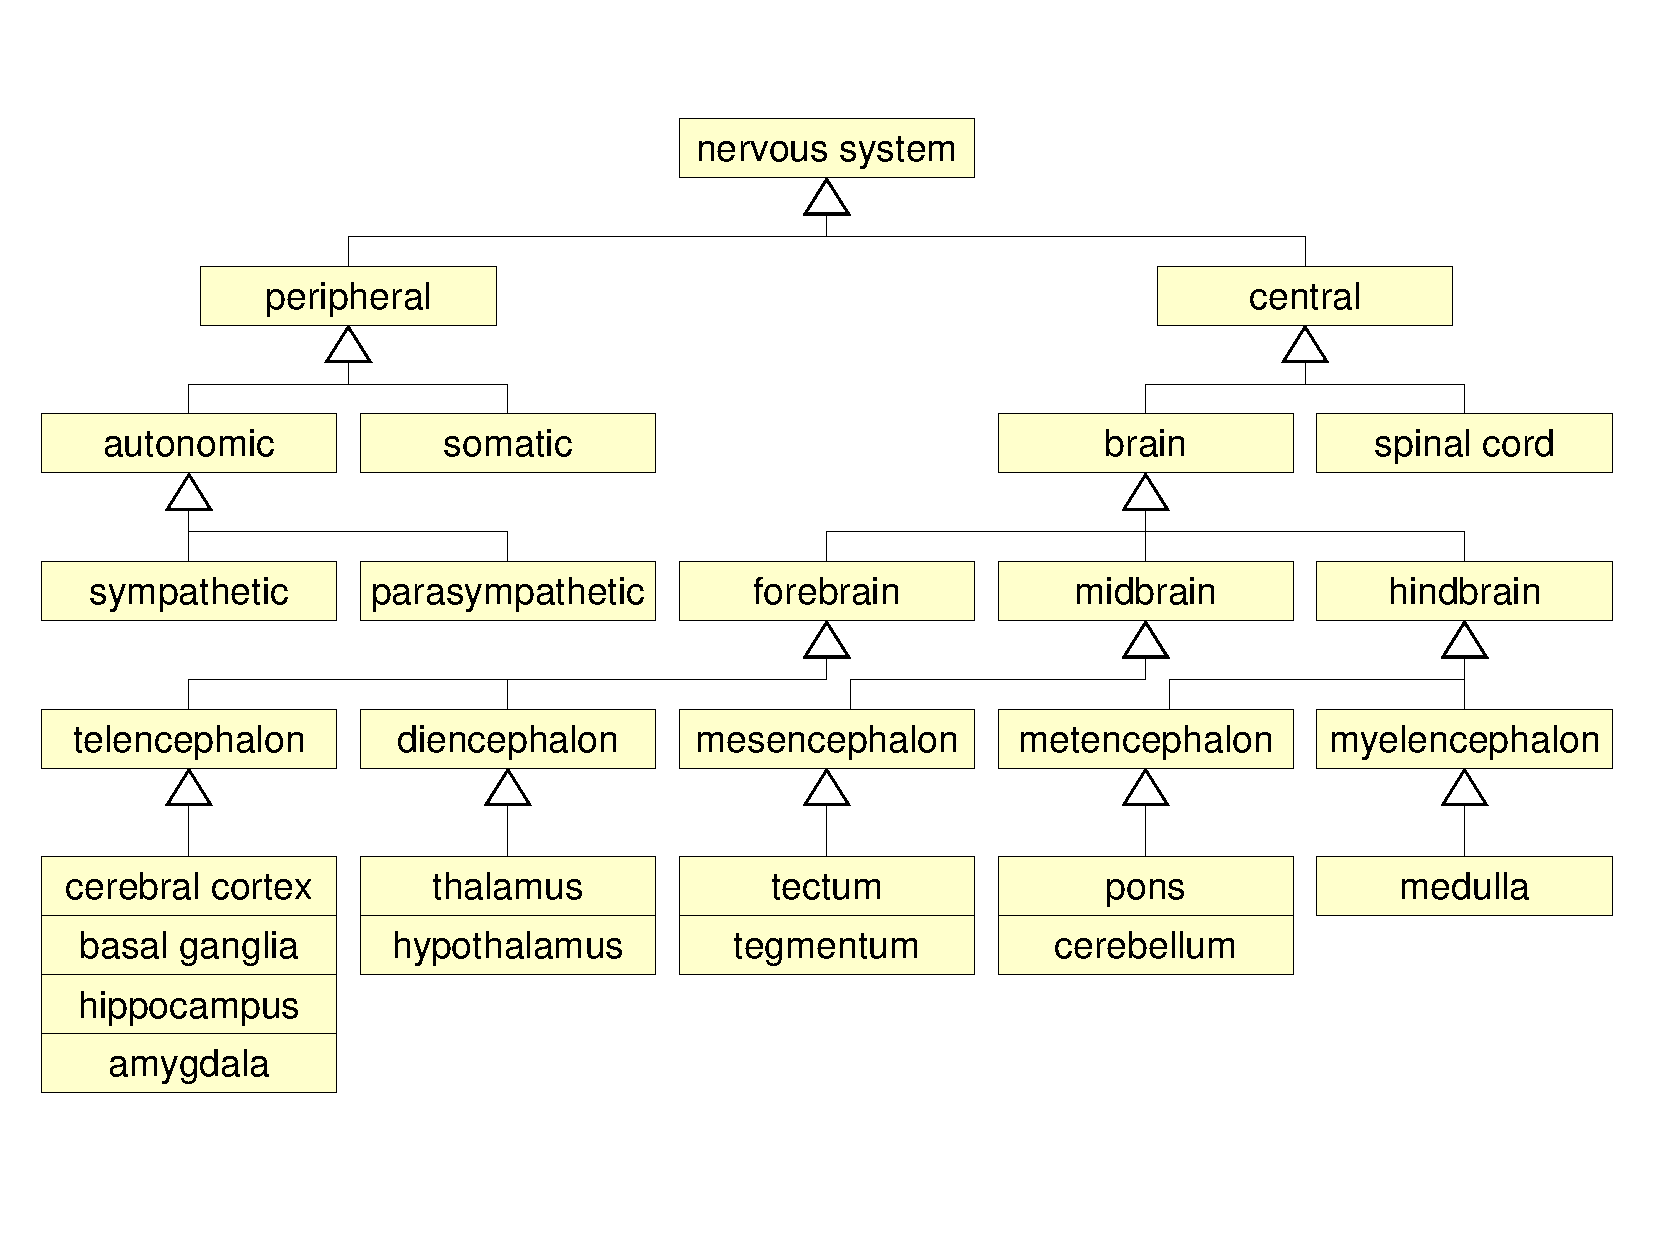
\includegraphics[scale=0.3,angle=-90]{graphic/nervoussystem.pdf}
        \caption{Divisions of the Nervous System \cite{adventuresinneuroanatomy}}
        \label{nervoussystem_figure}
    \end{center}
\end{figure}

Not all parts of this systematics shall be explained here; more details can be
found at \cite{pschyrembel}. Chapter \ref{state_and_logic_heading} will make
some remarks on the PNS, whose \emph{Neurons} (nerve cells) can be functionally
divided into \emph{sensory} (\emph{afferent}) and \emph{motor}
(\emph{efferent}) ones. The functions of some brain structures, as part of the
CNS, are described in table \ref{brainstructures_table}. At the same time, this
table (where \emph{n/a} means \emph{not applicable}) tries to give possible
analogies to a standard computer system, whereby hardware as well as software
are considered.

\begin{table}[ht]
    \begin{center}
        \begin{footnotesize}
        \begin{tabular}{| p{25mm} | p{50mm} | p{30mm} |}
            \hline
            \textbf{Brain Structure} & \textbf{Function} & \textbf{Computer Analogon}\\
            \hline
            Cerebral Cortex
            & Thought, Voluntary Movement, Language, Reasoning, Perception
            & Application/ Domain Knowledge\\
            \hline
            Cerebellum
            & Movement, Balance, Posture
            & n/a (only in Robots)\\
            \hline
            Brain Stem %(medulla, pons, tectum, tegmentum)
            & Breathing, Heart Rate, Blood Pressure
            & Timer, Power Supply\\
            \hline
            Hypothalamus
            & Body Temperature, Hunger, Thirst, Emotions, Circadian Rhythms
            & Self-observing Sensors (Battery-/ CPU Status)\\
            \hline
            Thalamus
            & Sensory Processing, Information Forwarding, Movement
            %(cerebral cortex [forwards information] to other brain areas and spinal cord)
            & Event Mechanism, Signal Loop, IRQ Handler\\
            \hline
            Limbic System %(amygdala, hippocampus)
            & Emotions
            & Signal Priorities\\
            \hline
            Hippocampus
            & Learning, Memory
            & Knowledge Storage, RAM\\
            \hline
            Basal Ganglia %(globus pallidus, caudate nucleus,
            %subthalamic nucleus, putamen, substantia nigra)
            & Movement
            & n/a (only in Robots)\\
            \hline
            Midbrain %(superior/ inferior colliculi, red nucleus)
            & Vision, Audition, Eye- and Body Movement
            & I/O Device Drivers, Translation\\
            \hline
        \end{tabular}
        \end{footnotesize}
        \caption{Brain Structures in Analogy to a Computer \cite{adventuresinneuroanatomy}}
        \label{brainstructures_table}
    \end{center}
\end{table}

Of course, the analogies do not match exactly. Also, there are many functions
-- like \emph{Thought} or \emph{Emotions} -- that a computer cannot perform.
The important thing to notice, however, is that there are brain regions mainly
\emph{storing} (Hippocampus) and \emph{applying} knowledge (Cerebral Cortex) and
others \emph{coordinating} the input/ output (i/o) of that knowledge (Midbrain,
Basal Ganglia) in form of simplified information, through sensoric/ motoric
organs of the human body.

That is, what philosophy calls \emph{Mind} (section \ref{mind_and_body_heading})
is the \emph{Knowledge} that is anatomically-physically mainly situated in the
\emph{Hippocampus} and \emph{Cerebral Cortex}. And again, i/o control does not
only rely on hardware devices but also on the corresponding driver software and
signalling mechanism. To say it differently: The software that contains
application/ domain knowledge is to be treated \emph{separately} from system
control software.

%
% $RCSfile: cell_division.tex,v $
%
% Copyright (C) 2002-2008. Christian Heller.
%
% Permission is granted to copy, distribute and/or modify this document
% under the terms of the GNU Free Documentation License, Version 1.1 or
% any later version published by the Free Software Foundation; with no
% Invariant Sections, with no Front-Cover Texts and with no Back-Cover
% Texts. A copy of the license is included in the section entitled
% "GNU Free Documentation License".
%
% http://www.cybop.net
% - Cybernetics Oriented Programming -
%
% http://www.resmedicinae.org
% - Information in Medicine -
%
% Version: $Revision: 1.1 $ $Date: 2008-08-19 20:41:05 $ $Author: christian $
% Authors: Christian Heller <christian.heller@tuxtax.de>
%

\subsection{Cell Division}
\label{cell_division_heading}
\index{Cell Division}
\index{Desoxy Ribo Nucleic Acid}
\index{DNA}

Among other topics, \emph{Biology} -- as the science of life -- deals with the
\emph{Biological Cell}, as smallest structural and functional unit of all
living organisms. All types of cells have a \emph{Membrane}, which envelopes a
substance called \emph{Cytoplasm}, and \emph{Desoxy Ribo Nucleic Acid-} (DNA)
as well as \emph{Ribo Nucleic Acid} (RNA) molecules. A DNA molecule is, roughly
said, a chain of \emph{Chemical Bases}. The \emph{Order} in which bases are
placed determines the properties of (\emph{Proteins} of) a biological creature.
To the \emph{Organelles} contained in cytoplasm belong \cite{wikipedia}:

\begin{itemize}
    \item[-] \emph{Cell Nucleus}: housing the genetic information
    \item[-] \emph{Ribosomes}: producing proteins
    \item[-] \emph{Mitochondria} and \emph{Chloroplasts}: generating energy
    \item[-] \emph{Endoplasmic Reticulum} (ER) and \emph{Golgi Apparatus}:
        transporting macromolecules
    \item[-] \emph{Lysosomes} and \emph{Peroxisomes}: digesting
\end{itemize}

Multicellular organisms grow by a process called \emph{Cell Division}, in which
a \emph{Mother Cell} divides into two \emph{Daughter Cells}. The process differs
slightly between cell types, but mostly, the genetic information (DNA) is
replicated first, before the cell nucleus- and finally the whole cell divides,
whereby the genetic information is distributed equally to both new-born cells.
The new cells use the genetic information encoded in the DNA, to create new
organelles and to function correctly.

In a comparative consideration, the cell corpus may be equated with a computer
system, and the genetic information with the software which runs that system.
Each cell represents a system with different hardware but all cells
(in one-and-the-same biological creature) use the same configuration
information. In other words, the configuration information can be forwarded and
used in different hardware.

But, again, there is one thing to keep in mind: \emph{System control software
is not equal to application software.} The configuration information contained
in a DNA may well represent the building plan for all kinds of cells in a
biological organism -- but it is not \emph{controlling} those cells. Genetic
information in a DNA is \emph{passive}; in order to make use of it, some
\emph{active} mechanism must be employed. In a biological cell, it is the RNA
molecules which transmit the genetic information from the DNA
(via transcription) into proteins (by translation).

In a simplified view, one might say: \textit{The cell is built according to the
instructions read from the DNA.} The genetic information of the DNA may be
compared to the domain knowledge of a software application, or generally to
configuration information -- also that of an \emph{Operating System} (OS).
The RNA activity and other cell control mechanisms, on the other hand, are
comparable to signalling, control loops, or the device drivers of an OS.

%
% $RCSfile: short_and_long_term_memory.tex,v $
%
% Copyright (C) 2002-2008. Christian Heller.
%
% Permission is granted to copy, distribute and/or modify this document
% under the terms of the GNU Free Documentation License, Version 1.1 or
% any later version published by the Free Software Foundation; with no
% Invariant Sections, with no Front-Cover Texts and with no Back-Cover
% Texts. A copy of the license is included in the section entitled
% "GNU Free Documentation License".
%
% http://www.cybop.net
% - Cybernetics Oriented Programming -
%
% http://www.resmedicinae.org
% - Information in Medicine -
%
% Version: $Revision: 1.1 $ $Date: 2008-08-19 20:41:08 $ $Author: christian $
% Authors: Christian Heller <christian.heller@tuxtax.de>
%

\subsection{Short- and Long-Term Memory}
\label{short_and_long_term_memory_heading}
\index{Short-Term Memory}
\index{STM}
\index{Long-Term Memory}
\index{LTM}
\index{Sensory Memory}
\index{Psychology}
\index{Persistent Storage}
\index{Transient Storage}

It was previously worked out that there are brain regions mainly storing and
applying knowledge and others controlling the input/ output (i/o) and
manipulation of that knowledge. \emph{Learning}, \emph{Storage} and
\emph{Recall} of knowledge are main tasks of the human brain, which are studied
by the science of \emph{Psychology}.

Besides the \emph{persistent} storage in \emph{Long Term Memory} (LTM), the brain
is capable of storing \emph{transient} information in \emph{Short Term Memory}
(STM), the latter also being called \emph{primary} or \emph{active} memory
\cite{wikipedia}. An additional \emph{Sensory Memory} stores information arriving
directly from the corresponding organs. Figure \ref{memory_figure} tries to
classify \emph{some} types of memory, as described by psychology. It is not
more than a \emph{trial} because psychology itself is not sure about memory
classification and several theories exist.

\begin{figure}[ht]
    \begin{center}
        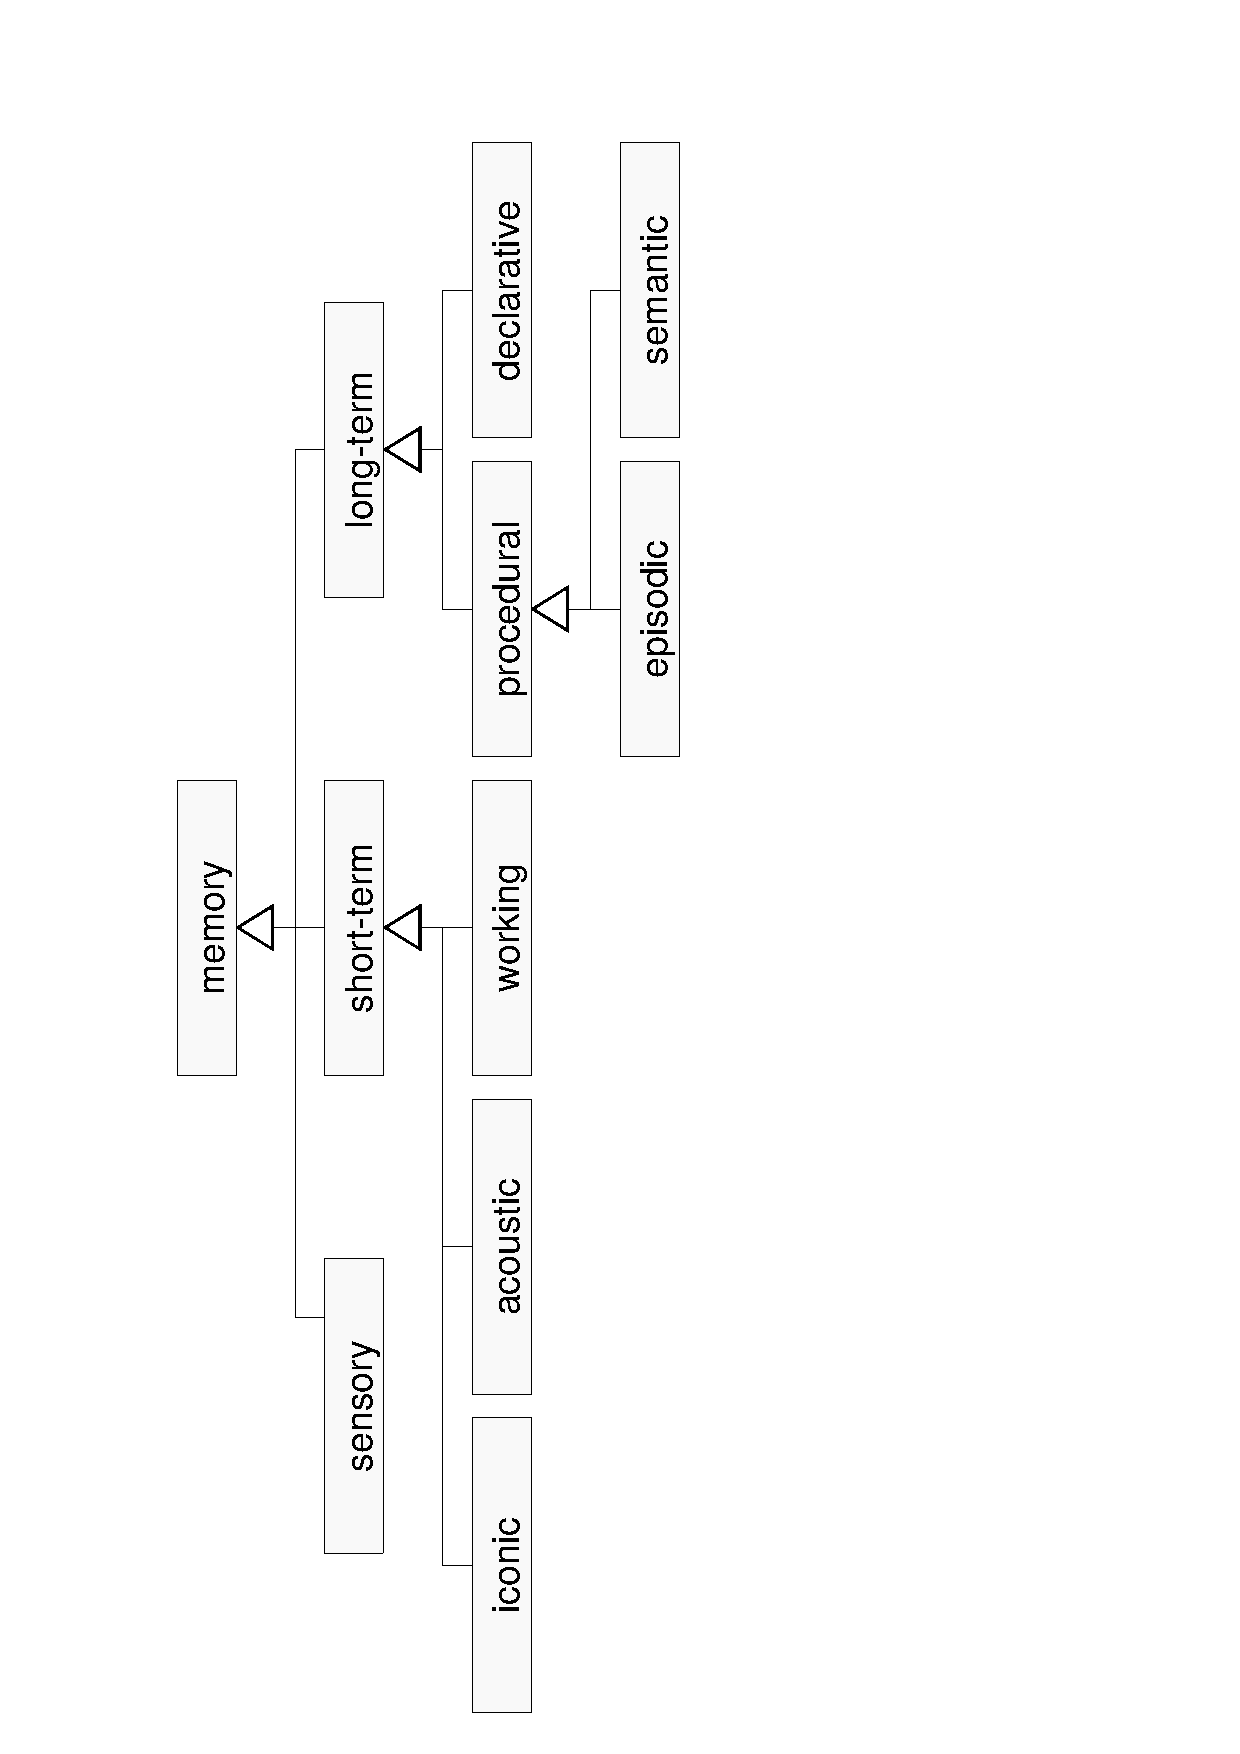
\includegraphics[scale=0.3,angle=-90]{graphic/memory.pdf}
        \caption{Types of Memory \cite{lai, eet}}
        \label{memory_figure}
    \end{center}
\end{figure}

The \emph{Encyclopedia of Educational Technology} (EET) \cite{eet} writes:

\begin{quote}
    The sensory information store has unlimited capacity, and reacts to both
    visual and auditory information. However, the duration of information in
    sensory memory is extremely brief, perhaps only 300 miliseconds, and is
    subject to rapid decay.

    STM, in general, is characterized by a limited capacity of up to seven
    pieces of independent information, and in the brief duration of these items
    in STM, usually anywhere from three to 20 seconds. Additionally, decay
    appears to be the primary mechanism of memory loss in STM.

    LTM efficiently stores our knowledge about the world. It is important to
    contrast LTM with other types of memory and understand how it is
    structured. The knowledge we store in LTM affects our perceptions of the
    world, and influences what information in the environment we attend to. LTM
    provides the framework to which we attach new knowledge, and its properties
    have important implications for instructional design.
\end{quote}

In the words of the Free Wikipedia Encyclopedia \cite{wikipedia}, Information
held in STM may be: \textit{recently processed sensory input; items recently
retrieved from LTM; or the result of recent mental processing.} When doing
mathematical calculations, for example, intermediary results stored in STM are
available for only a short time and forgotten soon after.

The \emph{declarative} LTM is conscious memory, a \emph{film} of past contents
\cite{fernandez}. The \emph{procedural} -- or \emph{non-declarative} -- LTM is
unconscious memory which enables humans to carry out a task (like riding a
bicycle), without having to consciously control it. In other words, procedures
stored in non-declarative LTM are available- and may run as background program.

What effects do these reflections have on the design of software systems? The
storage and dynamic processing of static knowledge may firstly rely on at least
two different kinds of memory, one for \emph{persistent-} and another one for
\emph{transient} storage of knowledge; secondly, they may rely not only on one
main process controlling the system, but (as equivalent to procedural LTM)
employ a number of background processes solving special tasks.

%
% $RCSfile: information_processing_model.tex,v $
%
% Copyright (C) 2002-2008. Christian Heller.
%
% Permission is granted to copy, distribute and/or modify this document
% under the terms of the GNU Free Documentation License, Version 1.1 or
% any later version published by the Free Software Foundation; with no
% Invariant Sections, with no Front-Cover Texts and with no Back-Cover
% Texts. A copy of the license is included in the section entitled
% "GNU Free Documentation License".
%
% http://www.cybop.net
% - Cybernetics Oriented Programming -
%
% http://www.resmedicinae.org
% - Information in Medicine -
%
% Version: $Revision: 1.1 $ $Date: 2008-08-19 20:41:07 $ $Author: christian $
% Authors: Christian Heller <christian.heller@tuxtax.de>
%

\subsection{Information Processing Model}
\label{information_processing_model_heading}
\index{Information Processing Model}
\index{Chunking}

Information processing, from the view of \emph{Cognitive Psychology}, follows
the model shown in figure \ref{processing_figure}. General information has to
pass several stages before it becomes meaningful knowledge. The results of
processing stages are stored in different memories.

\begin{figure}[ht]
    \begin{center}
        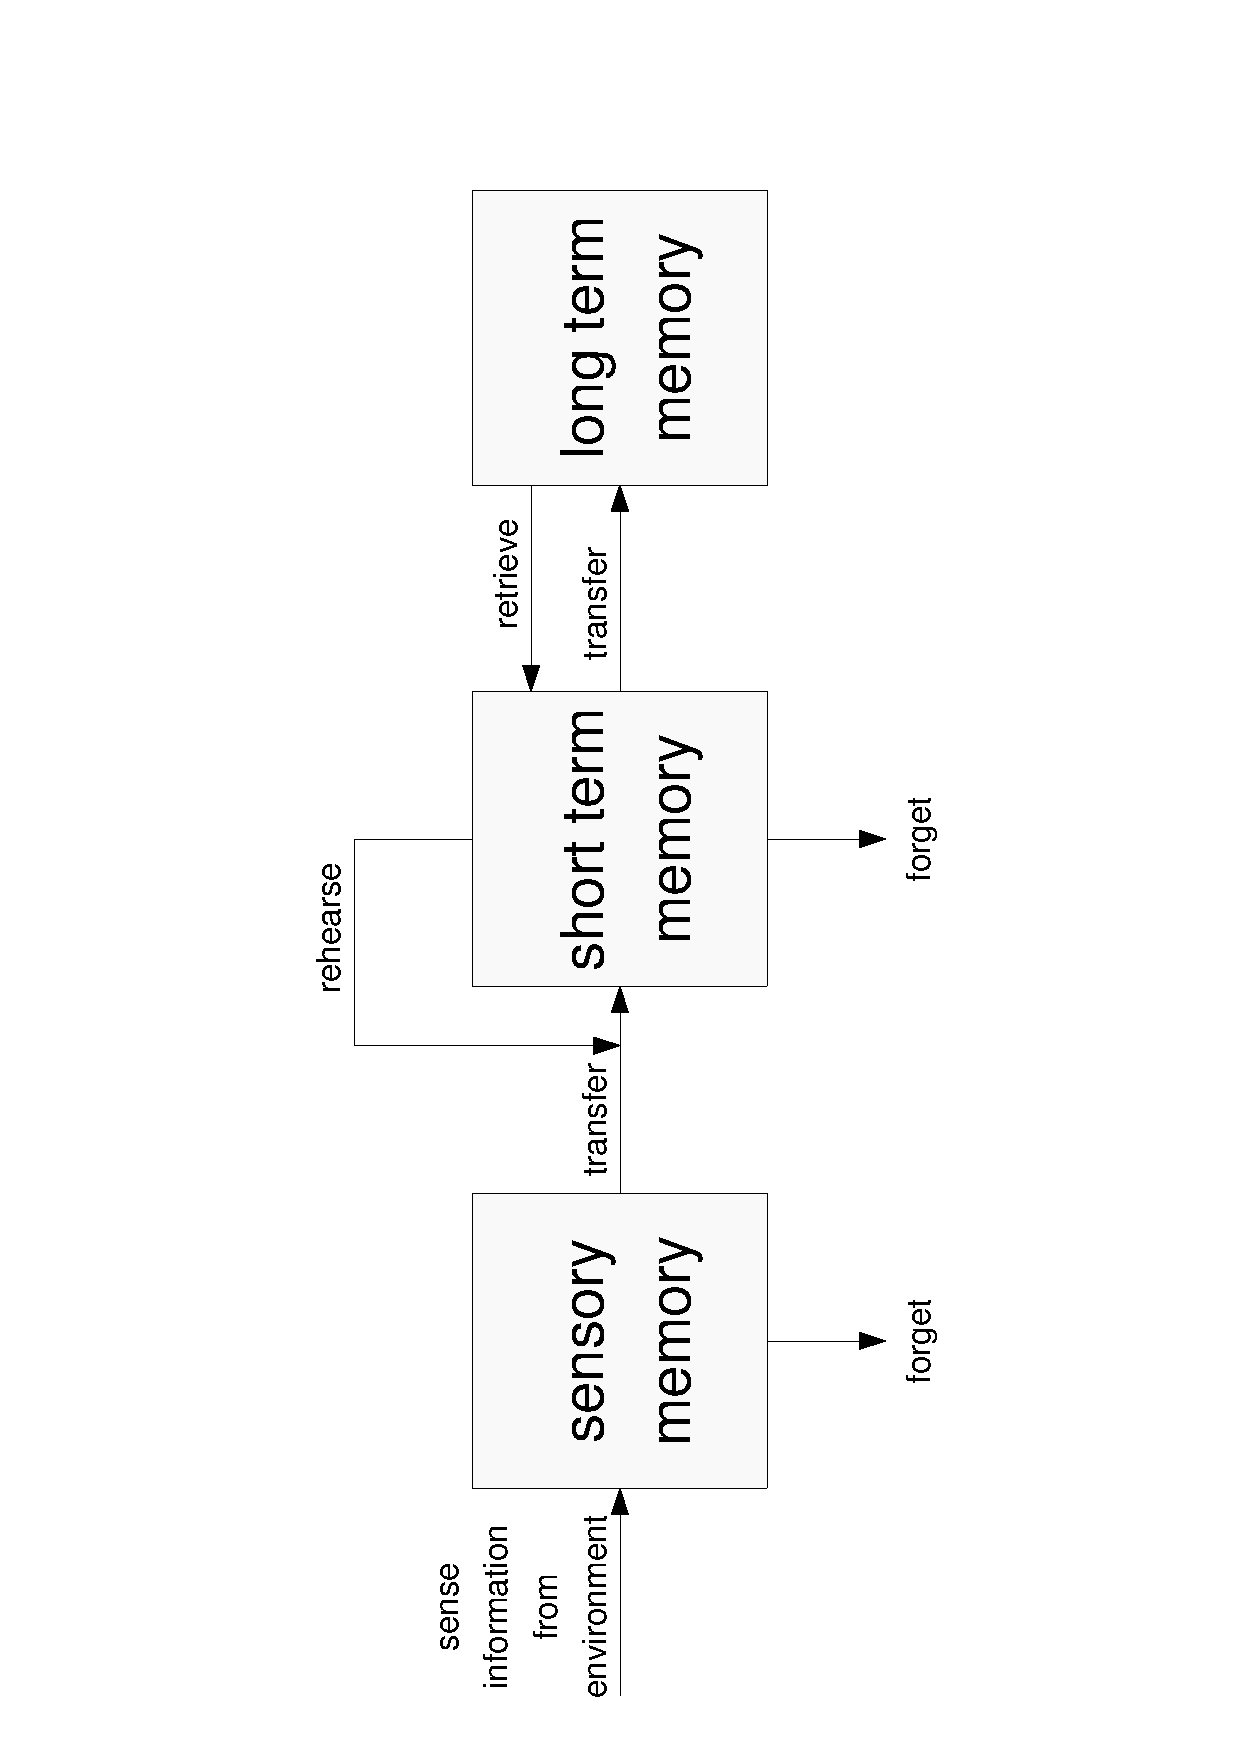
\includegraphics[scale=0.3,angle=-90]{graphic/processing.pdf}
        \caption{Information Processing Model \cite{eet}}
        \label{processing_figure}
    \end{center}
\end{figure}

The \emph{Encyclopedia of Educational Technology} (EET) \cite{eet} writes on
this:

\begin{quote}
    After entering sensory memory, a limited amount of information is
    transferred into short-term memory. \ldots\ The process of transferring
    information from STM into LTM involves the \emph{Encoding} or
    \emph{Consolidation} of information. \ldots\ Recent research (focuses) on
    the necessity of the brain to organise complex information in STM
    \emph{before} it can be encoded into LTM.

    In this process of organization, the \emph{Meaningfulness} or
    \emph{Emotional Content} of an item may play a greater role in its
    retention into LTM. Also, on a more concrete level, the use of
    \emph{Chunking} has been proven to be a significant aid to STM transfer to
    LTM. Because STM's capacity is limited to seven items, regardless of the
    complexity of those items, chunking allows the brain to automatically group
    certain items together.
\end{quote}

Certainly, the emotional content of an item can be neglected for computer
systems as of today. But chunking as a technique to divide information into
discrete items is of great importance in human thinking, which gets
investigated closer in chapter \ref{knowledge_schema_heading}.

%
% $RCSfile: persistent_and_transient.tex,v $
%
% Copyright (C) 2002-2008. Christian Heller.
%
% Permission is granted to copy, distribute and/or modify this document
% under the terms of the GNU Free Documentation License, Version 1.1 or
% any later version published by the Free Software Foundation; with no
% Invariant Sections, with no Front-Cover Texts and with no Back-Cover
% Texts. A copy of the license is included in the section entitled
% "GNU Free Documentation License".
%
% http://www.cybop.net
% - Cybernetics Oriented Programming -
%
% http://www.resmedicinae.org
% - Information in Medicine -
%
% Version: $Revision: 1.1 $ $Date: 2008-08-19 20:41:08 $ $Author: christian $
% Authors: Christian Heller <christian.heller@tuxtax.de>
%

\subsection{Persistent and Transient}
\label{persistent_and_transient_heading}
\index{Integrated Circuit}
\index{IC}
\index{Read Only Memory}
\index{ROM}
\index{Basic Input/ Output System}
\index{BIOS}
\index{Personal Digital Assistant}
\index{PDA}
\index{Electrically Erasable Programmable ROM}
\index{EEPROM}
\index{Flash ROM}
\index{Hard Disk Drive}
\index{HDD}
\index{Random Access Memory}
\index{RAM}
\index{Persistent Data}
\index{Transient Data}
\index{Volatile Data}
\index{Central Processing Unit}
\index{CPU}

In the science of \emph{Informatics}, there are a few \emph{Integrated Circuits}
(IC) -- so-called \emph{Read Only Memories} (ROM) -- containing unchangeable
programs. The \emph{Basic Input/ Output System} (BIOS) of a computer is one
example for such programs, software of \emph{Personal Digital Assistants} (PDA)
or \emph{Mobile Phones} are others. Often, the BIOS is stored in
\emph{Electrically Erasable Programmable ROM} (EEPROM) or its later form called
\emph{Flash ROM}. It thereby gets writable. When writing it, the complete old
BIOS gets overwritten. Most software programs, however, reside on a
\emph{Hard Disk Drive} (HDD) as permanent storage medium.

In order to use them, such \emph{persistent} programs often need to be loaded
into an IC called \emph{Random Access Memory} (RAM) which, other than a ROM,
can be both read from and written to. Most RAMs are \emph{volatile} which means
that the data they store -- to which also belong programs -- are
\emph{transient}, that is get lost in case the computer is powered down. The
ability to manipulate data in memory is a pre-requisite to usefully work with a
computer.

One surely could, with some effort, rearchitect computers so to let the
\emph{Central Processing Unit} (CPU) communicate directly with persistent
memory (like a HDD), instead of RAM. One reason for not doing this is the
\emph{Performance} of computer systems -- RAM can be accessed much faster than a
HDD. Another reason is the independence from differing HDD designs.

What this section by its remarks tries to show is that \emph{static} software
becomes \emph{dynamic}, that is changeable over time, when being loaded into a
RAM whose data (represented by its state) can be processed (manipulated)
through a CPU. Although not being so new, this statement has importance for
some considerations later in this chapter.

While some kinds of software (like standard- or business applications) mainly
\emph{contain} static knowledge of a special domain, other kinds do mainly
\emph{use} that knowledge to dynamically control hardware. The point is that
traditionally, both kinds of software are mixed up. A business application has
to care about memory allocation, graphical input and output (even when using a
framework for that), communication mechanisms and more, although these are not
in its original interest. On the other hand, an operating system often contains
configuration knowledge about its structure or available devices that does not
actually belong into it. In order to achieve a clearer structure with less
dependencies and more flexibility, it is necessary to treat both kinds of
software differently.


%
% $RCSfile: system_and_knowledge.tex,v $
%
% Copyright (C) 2002-2008. Christian Heller.
%
% Permission is granted to copy, distribute and/or modify this document
% under the terms of the GNU Free Documentation License, Version 1.1 or
% any later version published by the Free Software Foundation; with no
% Invariant Sections, with no Front-Cover Texts and with no Back-Cover
% Texts. A copy of the license is included in the section entitled
% "GNU Free Documentation License".
%
% http://www.cybop.net
% - Cybernetics Oriented Programming -
%
% http://www.resmedicinae.org
% - Information in Medicine -
%
% Version: $Revision: 1.1 $ $Date: 2008-08-19 20:41:09 $ $Author: christian $
% Authors: Christian Heller <christian.heller@tuxtax.de>
%

\section{System and Knowledge}
\label{system_and_knowledge_heading}
\index{System and Knowledge}

Having explained why a strict separation of application knowledge and system
control software is desirable, several state-of-the-art techniques can now be
considered once again, in order to find out about possible new effects to
software design or source code.

%
% $RCSfile: configurable_or_programmable.tex,v $
%
% Copyright (C) 2002-2008. Christian Heller.
%
% Permission is granted to copy, distribute and/or modify this document
% under the terms of the GNU Free Documentation License, Version 1.1 or
% any later version published by the Free Software Foundation; with no
% Invariant Sections, with no Front-Cover Texts and with no Back-Cover
% Texts. A copy of the license is included in the section entitled
% "GNU Free Documentation License".
%
% http://www.cybop.net
% - Cybernetics Oriented Programming -
%
% http://www.resmedicinae.org
% - Information in Medicine -
%
% Version: $Revision: 1.1 $ $Date: 2008-08-19 20:41:06 $ $Author: christian $
% Authors: Christian Heller <christian.heller@tuxtax.de>
%

\subsection{Configurable or Programmable}
\label{configurable_or_programmable_heading}
\index{Configurable System}
\index{Programmable System}
\index{Key-Value-Pair}
\index{Knowledge}
\index{External Knowledge}
\index{Operating System}
\index{OS}

\emph{Knowledge} (first defined in section \ref{knowledge_engineering_heading}
of this work) is present in all kinds of software systems. It is what
characterises a system, because: it defines possible states and logic, their
structure and relations, and thereby a complete application; it such determines
the way a system process controls the computer hardware it runs on; it thereby
has the capability to change the properties and behaviour of a whole computer
system. One can therefore say that knowledge encoded in software represents the
\emph{Configuration} information necessary to run a computer system in the
desired way.

In addition to the configuration information hard-coded in the program, most
applications offer to alter special settings such as paths, language choice and
spelling, editor and saving options, colours, fonts and further properties.
Usually, these are made persistent using some kind of external storage like a
flat file or a database. One popular format for storing simple properties are
so-called \emph{Key-Value-Pairs}. Modern applications do also make use of
hierarchical storage for more complex settings.

Yet if a software program already represents all knowledge needed to run an
application on a computer, why storing extra settings externally? Obviously, a
standard program is not \emph{flexible} enough; it cannot be changed anymore
after compilation. But program changes at runtime are often highly desirable.

So, if external storage of properties does make sense, why not storing
\emph{everything} outside the actual program? This seems to be a crazy but very
useful idea, as it would result in absolutely flexible application systems. But
it has limits. There \emph{must} be some core program (\emph{Kernel}) able to
read and write (\emph{interpret}), and to process (\emph{handle}) external
properties (\emph{Signals}). The more complex, structured and inter-related
these properties are, the more suitable it is to call them \emph{Knowledge}.

A technical system may be able to understand external knowledge, just like
human beings have the cognitive abilities to understand their environment by
building a \emph{Virtual World} of it. Yet is this not enough. Knowledge about
the \emph{Real World} environment is one thing; interacting with it another. A
computer has hardware devices for interacting with the real world. The devices
need to be operated correctly so that knowledge can be exchanged through them.
This hardware driving functionality is normally provided by an
\emph{Operating System} (OS). But current OS have the deficiency of not being
able to handle knowledge. What is needed, finally, is a system with
\emph{low-level} hardware control abilities like an operating system
\emph{plus} additional \emph{high-level} knowledge handling abilities
\cite{heller2004}.

Other people reflected on this and have come to a similar conclusion. Thomas
Beale writes in \cite{openhealth}:

\begin{quote}
    The history of IT \ldots\ has taught us that the only kind of useful system
    that can be delivered to domain users \ldots\ is one which is not just
    configurable, but \emph{programmable} -- not by statements of source code,
    but by high-level \emph{domain-user-oriented} tools.
\end{quote}

Well, the user-oriented, domain-knowledge handling tools are desirable, but only
in the second place. The important part of this statement is the realisation that
systems need to become \emph{programmable}, and this by \emph{External Knowledge}.
Whether this knowledge gets created and maintained manually or by using graphical
tools, is of minor importance. What is needed in any case is a formal knowledge
specification language serving as basis for the people or tools to work on.
Chapter \ref{cybernetics_oriented_language_heading} will introduce such a
language.

%
% $RCSfile$
%
% Copyright (c) 2002-2006. Christian Heller. All rights reserved.
%
% Permission is granted to copy, distribute and/or modify this document
% under the terms of the GNU Free Documentation License, Version 1.1 or
% any later version published by the Free Software Foundation; with no
% Invariant Sections, with no Front-Cover Texts and with no Back-Cover
% Texts. A copy of the license is included in the section entitled
% "GNU Free Documentation License".
%
% http://www.cybop.net
% - Cybernetics Oriented Programming -
%
% http://www.resmedicinae.org
% - Information in Medicine -
%
% Version: $Revision$ $Date$ $Author$
% Authors: Christian Heller <christian.heller@tuxtax.de>
%

\subsubsection{Code Reduction}
\label{code_reduction_heading}

In his book \emph{Programming Pearls} \cite[page 128]{bentley}, Jon Bentley
demonstrates \emph{Code Reduction} on the following graphics program example:

\begin{scriptsize}
    \begin{verbatim}
� � for i = [17, 43] set(i, 68)
� � for i = [18, 42] set(i, 69)
� � for j = [81, 91] set(30, j)
� � for j = [82, 92] set(31, j)
    \end{verbatim}
\end{scriptsize}

He suggests to replace the \emph{set} procedures that switch a
\emph{Picture Element} (Pixel) with suitable functions for drawing horizontal
and vertical lines:

\begin{scriptsize}
    \begin{verbatim}
� � hor(17, 43, 68)
� � hor(18, 42, 69)
� � vert(81, 91, 30)
� � vert(82, 92, 31)
    \end{verbatim}
\end{scriptsize}

This code, finally, gets reduced to pure data stored in an array:

\begin{scriptsize}
    \begin{verbatim}
� � h 17 43 68
� � h 18 42 69
� � v 81 91 30
� � v 82 92 31
    \end{verbatim}
\end{scriptsize}

The data can be read by an interpreter program which knows about their meaning.

Bentley's example shows in a nice way how knowledge can be extracted from program
source code. The graphic application's actual data are represented by the values
in the array above. All other functionality accessing and manipulating Pixels
directly does belong to system control and remains in the interpreter program.
Section \ref{cyboi_heading} will introduce an interpreter that is able to read
and handle \emph{general} knowledge, only on a much larger scale.

%
% $RCSfile: base_and_meta_level.tex,v $
%
% Copyright (C) 2002-2008. Christian Heller.
%
% Permission is granted to copy, distribute and/or modify this document
% under the terms of the GNU Free Documentation License, Version 1.1 or
% any later version published by the Free Software Foundation; with no
% Invariant Sections, with no Front-Cover Texts and with no Back-Cover
% Texts. A copy of the license is included in the section entitled
% "GNU Free Documentation License".
%
% http://www.cybop.net
% - Cybernetics Oriented Programming -
%
% http://www.resmedicinae.org
% - Information in Medicine -
%
% Version: $Revision: 1.1 $ $Date: 2008-08-19 20:41:05 $ $Author: christian $
% Authors: Christian Heller <christian.heller@tuxtax.de>
%

\subsection{Base- and Meta Level}
\label{base_and_meta_level_heading}
\index{Base Level}
\index{Meta Level}
\index{Reflective Technique}
\index{System- and Application Functionality}
\index{Bidirectional Dependency}

Reflective techniques as described in section \ref{reflection_heading} make use
of one so-called \emph{Base Level} and one or more \emph{Meta Levels}. The
reason for splitting a system's architecture in this way is the hope to be able
to move rather general \emph{System Functionality} into a meta level, while
leaving domain-specific \emph{Application Functionality} in the base level.
(Well, in his book \emph{Analysis Patterns -- Reusable Object Models}
\cite{fowler1997}, Fowler used meta levels to model general classes containing
not exclusively system- but also domain-specific functionality.) The conflicts
a design decision of that kind can bring with were described in section
\ref{broken_type_system_heading}, which -- above all -- criticised the
bidirectional dependencies.

However, what the proposition of reflective software patterns shows, is the
existence of a wish among software developers, to separate general system- from
more specific application functionality. And, as was shown in section
\ref{virtual_and_real_world_heading}, nature does exactly that. Yet while
reflective mechanisms use the same implementation techniques for system- as
well as for application-specific functionality, nature always treats passive
knowledge strictly separate from active system control (section
\ref{virtual_and_real_world_heading}). Bidirectional dependencies do not exist
between the both.

%
% $RCSfile: reference_and_archetype_model.tex,v $
%
% Copyright (C) 2002-2008. Christian Heller.
%
% Permission is granted to copy, distribute and/or modify this document
% under the terms of the GNU Free Documentation License, Version 1.1 or
% any later version published by the Free Software Foundation; with no
% Invariant Sections, with no Front-Cover Texts and with no Back-Cover
% Texts. A copy of the license is included in the section entitled
% "GNU Free Documentation License".
%
% http://www.cybop.net
% - Cybernetics Oriented Programming -
%
% http://www.resmedicinae.org
% - Information in Medicine -
%
% Version: $Revision: 1.1 $ $Date: 2008-08-19 20:41:08 $ $Author: christian $
% Authors: Christian Heller <christian.heller@tuxtax.de>
%

\subsection{Reference- and Archetype Model}
\label{reference_and_archetype_model_heading}
\index{Reference Model}
\index{RM}
\index{Archetype Model}
\index{AM}
\index{Archetype}
\index{Archetype Definition Language}
\index{ADL}
\index{Dual Model Approach}

The \emph{Archetype} concept as introduced in section \ref{archetype_heading}
\emph{does} provide an independent implementation technique (language) for the
definition of application-specific domain knowledge: the
\emph{Archetype Definition Language} (ADL). The documents written in it,
altogether, are referred to as \emph{Archetype Model} (AM). They get parsed and
instantiated at runtime. These instances are then used to constrain instances
of a \emph{Reference Model} (RM). Because of the existence of two models
implemented with two independent techniques, this method of programming is
called \emph{Dual Model Approach} (section \ref{dual_model_approach_heading}).

It wants to solve the dilemma of lacking domain semantics in classical
information models. Archetypes are the corresponding knowledge documents
carrying semantic information. They provide the structures and rules after
which instances of an RM can be combined meaningfully. Despite its drawbacks
mentioned in section \ref{dual_model_approach_heading}, the dual model approach
animated this work to pay attention to two things:

\begin{enumerate}
    \item the usage of different implementation technologies for domain
        knowledge (AM) and underlying system-level functionality (RM)
    \item the need to provide constraint information with knowledge models
\end{enumerate}

The distinction between domain knowledge and system-level functionality is
realised by providing a knowledge modelling language (chapter
\ref{cybernetics_oriented_language_heading}) and a corresponding interpreter
(chapter \ref{cybernetics_oriented_interpreter_heading}). The language is
capable of expressing structural- as well as meta information, to which also
belong constraints.

%
% $RCSfile: common_and_crosscutting_concerns.tex,v $
%
% Copyright (C) 2002-2008. Christian Heller.
%
% Permission is granted to copy, distribute and/or modify this document
% under the terms of the GNU Free Documentation License, Version 1.1 or
% any later version published by the Free Software Foundation; with no
% Invariant Sections, with no Front-Cover Texts and with no Back-Cover
% Texts. A copy of the license is included in the section entitled
% "GNU Free Documentation License".
%
% http://www.cybop.net
% - Cybernetics Oriented Programming -
%
% http://www.resmedicinae.org
% - Information in Medicine -
%
% Version: $Revision: 1.1 $ $Date: 2008-08-19 20:41:05 $ $Author: christian $
% Authors: Christian Heller <christian.heller@tuxtax.de>
%

\subsection{Common- and Crosscutting Concerns}
\label{common_and_crosscutting_concerns_heading}
\index{Aspect Oriented Programming}
\index{AOP}
\index{Object Oriented Programming}
\index{OOP}
\index{Common Concern}
\index{Crosscutting Concern}
\index{Development Concern}
\index{Production Concern}
\index{Classification of Concerns}

Section \ref{aspect_oriented_programming_heading} argumented that, after
\cite{aspectj}, \emph{Aspect Oriented Programming} (AOP) were necessary because
some concerns were not easily turned into \emph{Classes} -- the natural unit of
modularity for \emph{Object Oriented Programming} (OOP) -- because they'd cut
across classes. Much like OOP were a way of modularising \emph{Common Concerns},
AOP were a way of modularising \emph{Crosscutting Concerns}. Figure
\ref{concerns_figure} is a trial to classify both kinds. (The distinction into
\emph{Development-} and \emph{Production Concerns} is of minor importance here.)

\begin{figure}[ht]
    \begin{center}
        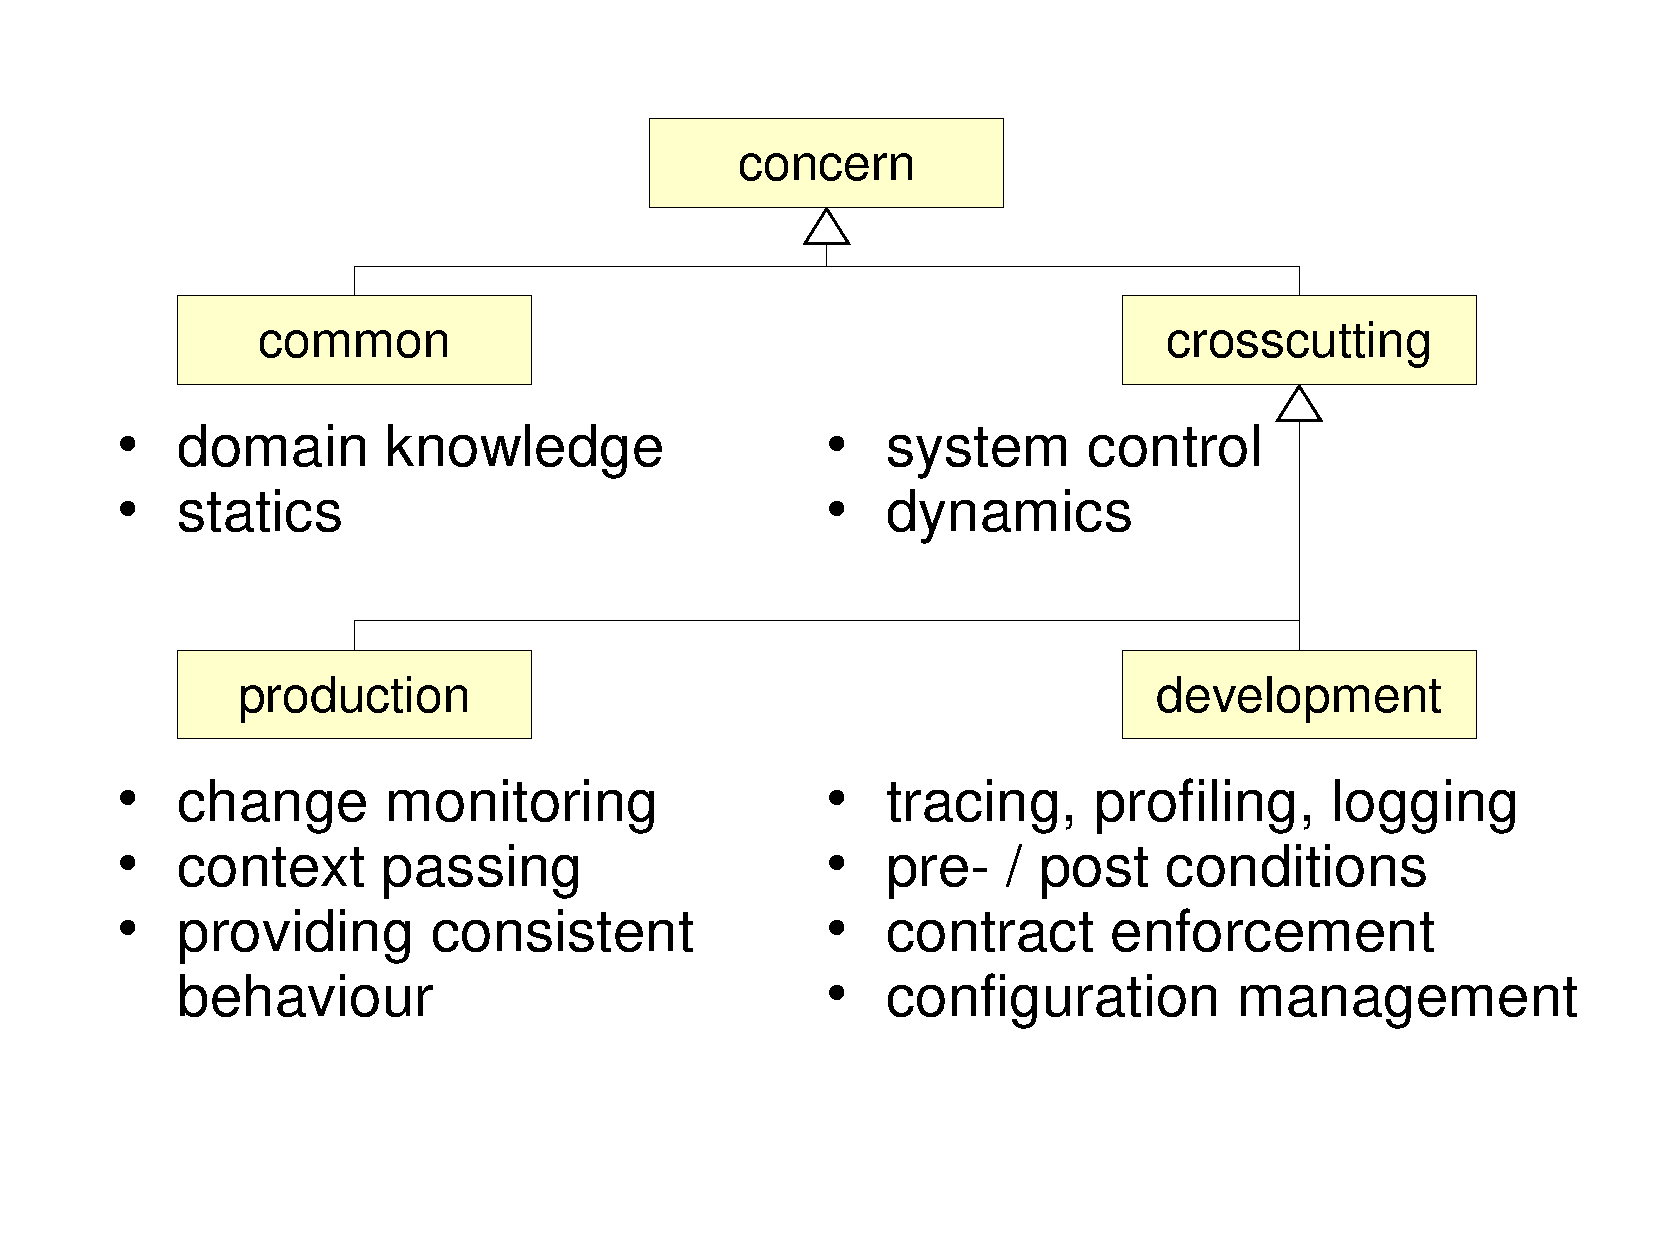
\includegraphics[scale=0.3,angle=-90]{graphic/concerns.pdf}
        \caption{Classification of Concerns}
        \label{concerns_figure}
    \end{center}
\end{figure}

Looking closer at these, it becomes obvious that crosscutting concerns represent
general \emph{System Control} functionality, while common concerns stand for
properties specific to an \emph{Application}. Comparing with nature (section
\ref{virtual_and_real_world_heading}), the separation of both kinds of concerns
seems absolutely correct. It arises the question, however, if AOP with all its
additional concepts is really the most suitable way for treating crosscutting
concerns? This work means \emph{no} and suggests to simply put all general
control functionality into a basic knowledge-interpreter system underlying all
applications (chapter \ref{cybernetics_oriented_interpreter_heading}).

%
% $RCSfile$
%
% Copyright (c) 2005-2006. Christian Heller. All rights reserved.
%
% Permission is granted to copy, distribute and/or modify this document
% under the terms of the GNU Free Documentation License, Version 1.1 or
% any later version published by the Free Software Foundation; with no
% Invariant Sections, with no Front-Cover Texts and with no Back-Cover
% Texts. A copy of the license is included in the section entitled
% "GNU Free Documentation License".
%
% http://www.cybop.net
% - Cybernetics Oriented Programming -
%
% http://www.resmedicinae.org
% - Information in Medicine -
%
% Version: $Revision$ $Date$ $Author$
% Authors: Christian Heller <christian.heller@tuxtax.de>
%

\subsubsection{Application and Domain}
\label{application_and_domain_heading}

Over the years, it has turned out to be helpful in software design, to separate
\emph{Domain Knowledge} from \emph{Application Functionality}. In
one-or-another form, the architectural software patterns \cite{heller2005}
\emph{Layers}, \emph{Domain Model} and \emph{Model View Controller} (MVC) all
suggest to apply this principle.

The \emph{Tools \& Materials} approach \cite{tandm} talks of \emph{active}
applications (tools) working on \emph{passive} domain data (material). And also
\emph{System Family Engineering} \cite{domainengg} bases on a separate
treatment of domain and application, in form of \emph{Domain Engineering} (DE)
and \emph{Application Engineering} (AE).

An often neglected fact of these approaches is that not only the domain, but
also the application contains important business knowledge (figure
\ref{separation_figure}). The \emph{User Interface} (UI), for example, is
tailored for a specific business domain. And the logic behind, if not
contained in the UI itself, is often put in a \emph{Controller} which belongs
to the application$-$, not the domain layer.

\begin{figure}[ht]
    \begin{center}
        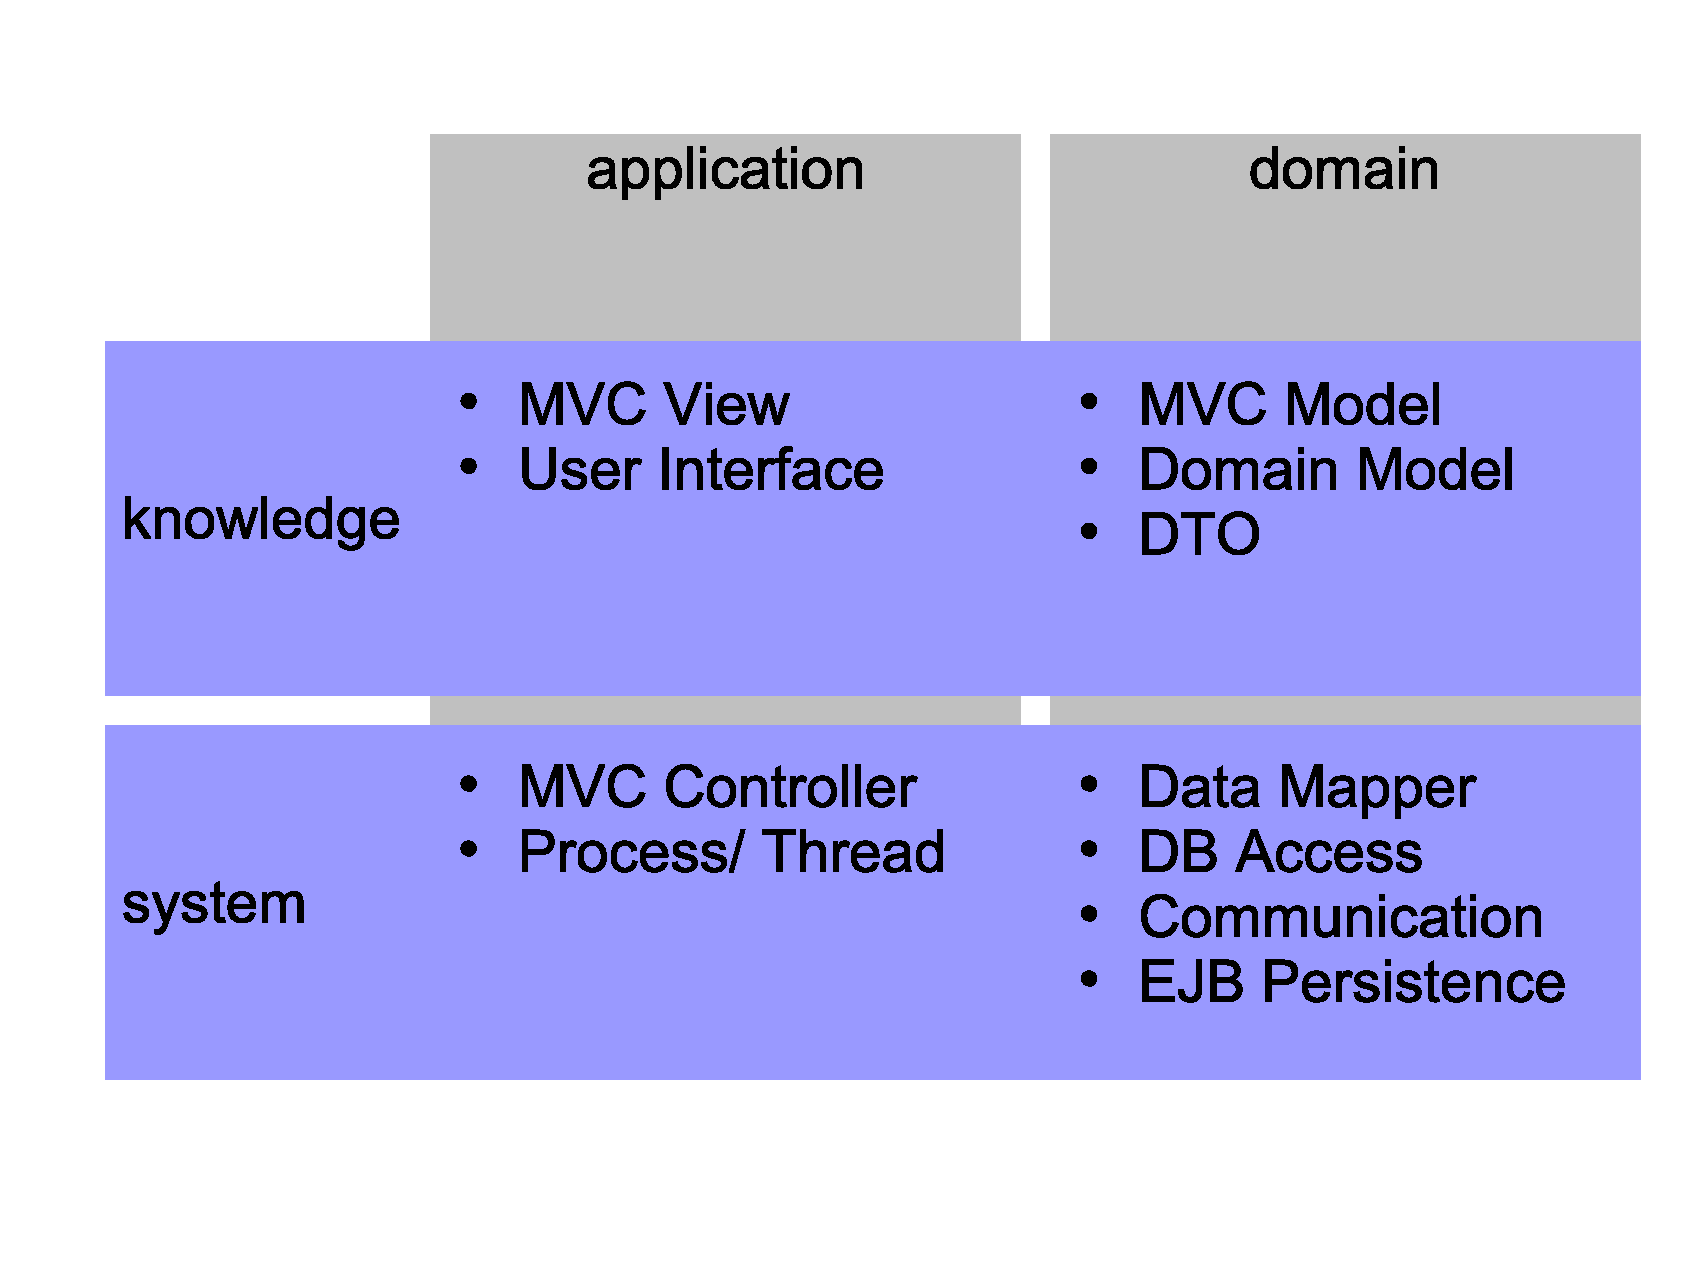
\includegraphics[scale=0.2]{vector/separation.eps}
        \caption{Different Knowledge Separations}
        \label{separation_figure}
    \end{center}
\end{figure}

Similarly, the domain often contains functionality which actually does belong
into the application process: \emph{Database} (DB) access is handled by help of
patterns like the \emph{Data Mapper} \cite{heller2005}, in which the mapper\\
objects contain \emph{Structured Query Language} (SQL) code to connect to a
\emph{Database Management System} (DBMS); \emph{Enterprise Java Beans} (EJB),
which should better be pure domain objects, imitate a \emph{Middleware}
providing persistence- or communication mechanisms, which originally have
nothing to do with the business knowledge they contain.

It is precisely this \emph{Mixup} of responsibilities between an application
system and its domain knowledge, that leads to multiple inter-dependencies and
hence unflexibility within a system. Instead, a separation should be made
between active \emph{System Control} and passive \emph{Knowledge}. A UI's
appearance would then be treated as domain knowledge, just as the logic of the
functions called through it. A data mapper would be transformed into a simple
\emph{Translator} -- similar to a \emph{Data Transfer Object} (DTO)
\cite{heller2005} -- that knows how to convert data from one domain model into
another; its DBMS access functionality, however, would be extracted and put
into the application system. Monstrosities like EJBs would likewise be opened
up and parted into their actual domain knowledge, and all other mechanisms
around -- the latter being moved into the application system.

To sum up this thought: The essential realisation here is that hardware-close
mechanisms like the ones necessary for data input/ output (i/o), enabling
inter-system communication, should be handled in an active application system
layer which was started as process on a computer, and \emph{not} be merged with
pure, passive domain knowledge. User interfaces and application logic which are
traditionally held in controller objects of the application layer, as well as
further business data models, should rather belong to a high-level knowledge
layer.

%
% $RCSfile$
%
% Copyright (c) 2002-2006. Christian Heller. All rights reserved.
%
% Permission is granted to copy, distribute and/or modify this document
% under the terms of the GNU Free Documentation License, Version 1.1 or
% any later version published by the Free Software Foundation; with no
% Invariant Sections, with no Front-Cover Texts and with no Back-Cover
% Texts. A copy of the license is included in the section entitled
% "GNU Free Documentation License".
%
% http://www.cybop.net
% - Cybernetics Oriented Programming -
%
% http://www.resmedicinae.org
% - Information in Medicine -
%
% Version: $Revision$ $Date$ $Author$
% Authors: Christian Heller <christian.heller@tuxtax.de>
%

\subsubsection{Platform Specific and -Independent}
\label{platform_specific_and_independent_heading}

The \emph{Model Driven Architecture} (MDA) \cite{mda} took a first step into
the right direction, by distinguishing \emph{Platform Independent Models}
(PIM), that is domain- and application logic, and \emph{Platform Specific Models}
(PSM), that is implementation technology. It encourages the use of automated
tools for defining and transforming these models.

While the definition, organisation and management of architectures (PIM) mostly
happen in the analysis- and design phase of a \emph{Software Engineering Process}
(SEP) (section \ref{abstraction_gaps_heading}), the generation of source code
(PSM) can be assigned to the implementation phase. The approach still has
weaknesses, and tools which can truly generate running systems are rare or not
existent, at least to what concerns more complex software systems -- not to
talk of the so-called \emph{Roundtrip Engineering}, which is managed by even
less tools.

Nevertheless, the trend clearly goes towards more model-centric approaches. The
aim of this work was to supply domain experts and application developers with a
\emph{Model Only} technology, allowing to create application systems that do
\emph{not} have to be transformed into classical implementation code any longer,
whereby the SEP abstraction gap number \emph{2} (figure \ref{gaps_figure})
could be closed conclusively. The knowledge schema introduced in section
\ref{knowledge_schema_heading} is a necessary prerequisite therefor.

%%
% $RCSfile: kernel_and_user_mode.tex,v $
%
% Copyright (C) 2002-2008. Christian Heller.
%
% Permission is granted to copy, distribute and/or modify this document
% under the terms of the GNU Free Documentation License, Version 1.1 or
% any later version published by the Free Software Foundation; with no
% Invariant Sections, with no Front-Cover Texts and with no Back-Cover
% Texts. A copy of the license is included in the section entitled
% "GNU Free Documentation License".
%
% http://www.cybop.net
% - Cybernetics Oriented Programming -
%
% http://www.resmedicinae.org
% - Information in Medicine -
%
% Version: $Revision: 1.1 $ $Date: 2008-08-19 20:41:07 $ $Author: christian $
% Authors: Christian Heller <christian.heller@tuxtax.de>
%

\subsection{Kernel- and User Mode}
\label{kernel_and_user_mode_heading}

Operating system: \cite[p. 249]{johnson}
1 user mode --> passive CYBOL knowledge
2 kernel mode --> active system control close to hardware

%
% $RCSfile: agent_with_mental_state.tex,v $
%
% Copyright (C) 2002-2008. Christian Heller.
%
% Permission is granted to copy, distribute and/or modify this document
% under the terms of the GNU Free Documentation License, Version 1.1 or
% any later version published by the Free Software Foundation; with no
% Invariant Sections, with no Front-Cover Texts and with no Back-Cover
% Texts. A copy of the license is included in the section entitled
% "GNU Free Documentation License".
%
% http://www.cybop.net
% - Cybernetics Oriented Programming -
%
% http://www.resmedicinae.org
% - Information in Medicine -
%
% Version: $Revision: 1.1 $ $Date: 2008-08-19 20:41:05 $ $Author: christian $
% Authors: Christian Heller <christian.heller@tuxtax.de>
%

\subsection{Agent with Mental State}
\label{agent_with_mental_state_heading}
\index{Agent Oriented Programming}
\index{AGOP}
\index{Agent}
\index{Mental State of an Agent}
\index{Formal Knowledge Representation Language of AGOP}
\index{Agent Programming Language of AGOP}
\index{Conversion Method of AGOP}

One design paradigm that early recognised the advantages of splitting software
into low-level system control and high-level knowledge, is
\emph{Agent Oriented Programming} (AGOP) (section
\ref{agent_oriented_programming_heading}). \emph{Agents}, as active software
components (which in this work means: \emph{running in an own process}), have
a \emph{Mental State} representing their knowledge, which they are able to
interpret and manipulate. This approach was copied in CYBOP.

Of the three elements \emph{Formal Knowledge Representation Language},
\emph{Agent Programming Language} and \emph{Conversion Method}, which an AGOP
system, after section \ref{agent_oriented_programming_heading}, needs in order
to be complete, this work provides the first two in form of the
\emph{Cybernetics Oriented Language} (CYBOL) and the
\emph{Cybernetics Oriented Interpreter} (CYBOI), described in sections
\ref{cybernetics_oriented_language_heading} and
\ref{cybernetics_oriented_interpreter_heading}, respectively. Thereby, CYBOI
itself is not a language, but represents a ready system, written in the
\emph{C} programming language. A method for converting traditional applications
into agents is not provided, since methodologies are clearly \emph{not} a topic
of this work.

Of course, there are differences distinguishing
\emph{Cybernetics Oriented Programming} (CYBOP) from traditional AGOP systems.
CYBOP needs an own interpreter, because of its new knowledge representation
philosophy and -language, which are the topic of chapters
\ref{knowledge_schema_heading} and \ref{cybernetics_oriented_language_heading}.
One reason for the difficult handling and intransparency of many traditional
knowledge representation languages is that they mix two kinds of knowledge:
\emph{State-} and \emph{Logic} descriptions. More on how this is avoided in
CYBOP in chapter \ref{state_and_logic_heading}.

One may wonder why such a supposedly advantageous architecture is not used by
all of today's systems? One reason may be that AGOP is still a rather young
technology lacking the necessary popularity. Another reason may be the bad
reputation of AGOP systems (and just about everything that has to do with
knowledge representation) among average developers -- partly because of their
immaturity, but mostly because of their complicated knowledge models and
-handling. Looking at the often quite cryptic appearance of the corresponding
languages, one tends to understand the developers' dislike.

%
% $RCSfile$
%
% Copyright (c) 2005-2006. Christian Heller. All rights reserved.
%
% Permission is granted to copy, distribute and/or modify this document
% under the terms of the GNU Free Documentation License, Version 1.1 or
% any later version published by the Free Software Foundation; with no
% Invariant Sections, with no Front-Cover Texts and with no Back-Cover
% Texts. A copy of the license is included in the section entitled
% "GNU Free Documentation License".
%
% http://www.cybop.net
% - Cybernetics Oriented Programming -
%
% http://www.resmedicinae.org
% - Information in Medicine -
%
% Version: $Revision$ $Date$ $Author$
% Authors: Christian Heller <christian.heller@tuxtax.de>
%

\subsubsection{Data Garden}
\label{data_garden_heading}

Now, if a distinction of high-level knowledge from low-level system control
software is considered to be useful, the next question must be: \textit{How,
that is in which form, best to store knowledge in a system?}

One possible structure called \emph{Data Garden} \cite{holland} was proposed by
Wau Holland of the \emph{Chaos Computer Club} (CCC). Although being a
non-academic organisation, his ideas on knowledge modelling are interesting to
this work. He dreamt of whole \emph{Forests}, \emph{Parks} or -- as the name
says -- \emph{Gardens} of \emph{Knowledge Trees} and \emph{Data Bushes} (figure
\ref{garden_figure}).

\begin{figure}[ht]
    \begin{center}
        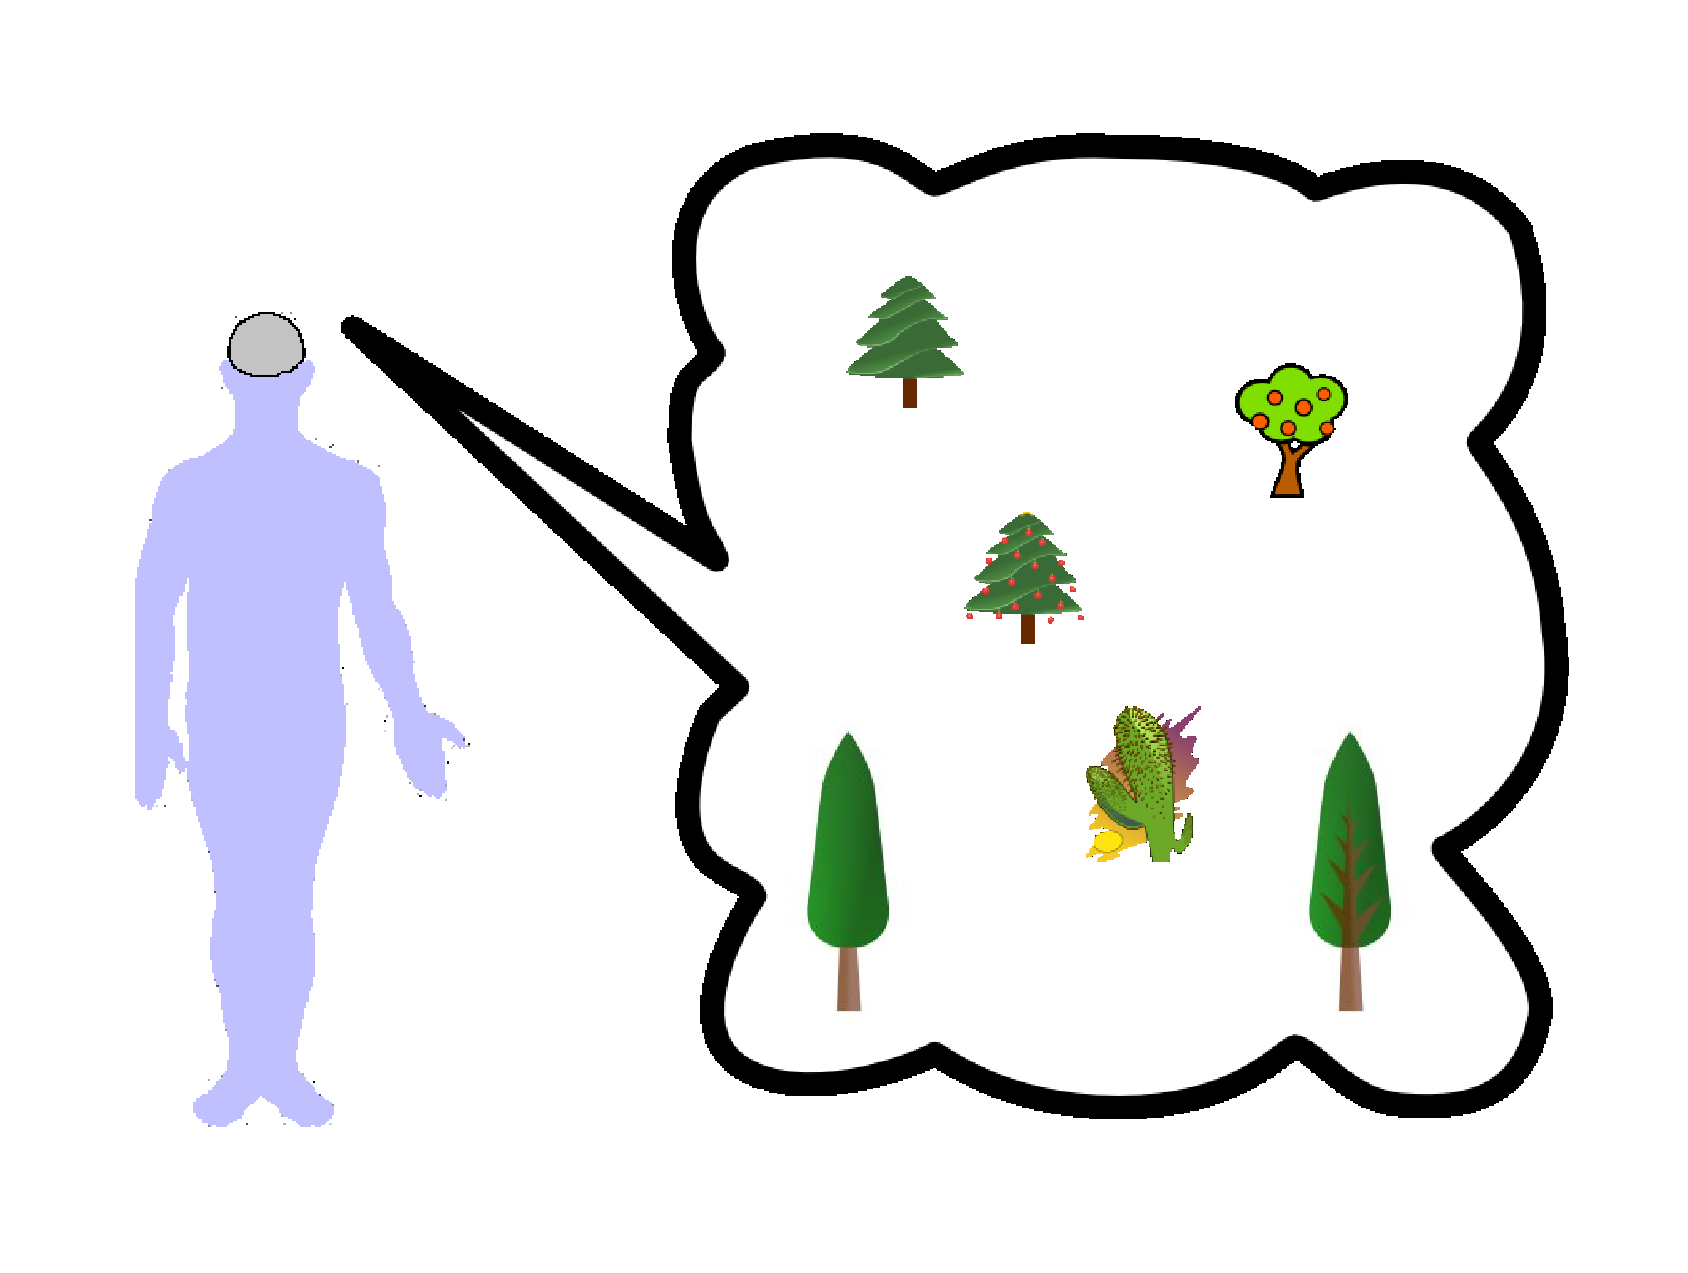
\includegraphics[scale=0.2]{vector/garden.eps}
        \caption{Data Garden}
        \label{garden_figure}
    \end{center}
\end{figure}

The interpreter (section \ref{cyboi_heading}) created in the work described in
this article stores all its knowledge in \emph{one single} tree, whose root
node it references. The single concepts (data bushes) are represented by
branches of that knowledge tree.


%
% $RCSfile: knowledge_management_system.tex,v $
%
% Copyright (C) 2002-2008. Christian Heller.
%
% Permission is granted to copy, distribute and/or modify this document
% under the terms of the GNU Free Documentation License, Version 1.1 or
% any later version published by the Free Software Foundation; with no
% Invariant Sections, with no Front-Cover Texts and with no Back-Cover
% Texts. A copy of the license is included in the section entitled
% "GNU Free Documentation License".
%
% http://www.cybop.net
% - Cybernetics Oriented Programming -
%
% http://www.resmedicinae.org
% - Information in Medicine -
%
% Version: $Revision: 1.1 $ $Date: 2008-08-19 20:41:07 $ $Author: christian $
% Authors: Christian Heller <christian.heller@tuxtax.de>
%

\section{Knowledge Management System}
\label{knowledge_management_system_heading}
\index{Knowledge Management System}

Section \ref{virtual_and_real_world_heading} justified a separation of knowledge
from system control software. Section \ref{system_and_knowledge_heading}
considered the effects of that separation to traditional software design. What
remains to be investigated is how a system adhering to a separation of that
kind would have to look like.

%
% $RCSfile: hardware_connection.tex,v $
%
% Copyright (C) 2002-2008. Christian Heller.
%
% Permission is granted to copy, distribute and/or modify this document
% under the terms of the GNU Free Documentation License, Version 1.1 or
% any later version published by the Free Software Foundation; with no
% Invariant Sections, with no Front-Cover Texts and with no Back-Cover
% Texts. A copy of the license is included in the section entitled
% "GNU Free Documentation License".
%
% http://www.cybop.net
% - Cybernetics Oriented Programming -
%
% http://www.resmedicinae.org
% - Information in Medicine -
%
% Version: $Revision: 1.1 $ $Date: 2008-08-19 20:41:07 $ $Author: christian $
% Authors: Christian Heller <christian.heller@tuxtax.de>
%

\subsection{Hardware Connection}
\label{hardware_connection_heading}
\index{Knowledge-Hardware Connection}
\index{Operating System}
\index{OS}
\index{Daemon}
\index{Knowledge}
\index{Control Software}
\index{Hardware}

Knowledge is \emph{passive}. What makes use of knowledge is the \emph{active}
parts of a system, in the case of computers a process like the
\emph{Operating System} (OS) or applications using external configuration
settings. They are able to both, communicate with hardware and adopt knowledge,
for it to be memorised and processed.

Traditionally, OS make use of a number of helper processes (\emph{Daemons},
section \ref{local_process_heading}), for services like printing or email
delivery, which may also be used by applications. This work, however, wants to
unify services in just one low-level system control process. Another issue are
the varying communication paradigms a classical application has to consider.
Persistence mechanisms, user interfaces, remote communication -- they all have
their specific requirements, whether supported by a special framework (section
\ref{framework_heading}) or not. This work wants to simplify communication in a
way that applications do not have to do more than issuing a simple \emph{send}
or \emph{receive} instruction, adding the desired language of communication. By
disburdening applications from low-level communication and signal (event)
handling responsibilities, they become purely passive knowledge (statics) which
cannot act itself, but needs to be read and interpreted by an active control
process (dynamics).

\begin{figure}[ht]
    \begin{center}
        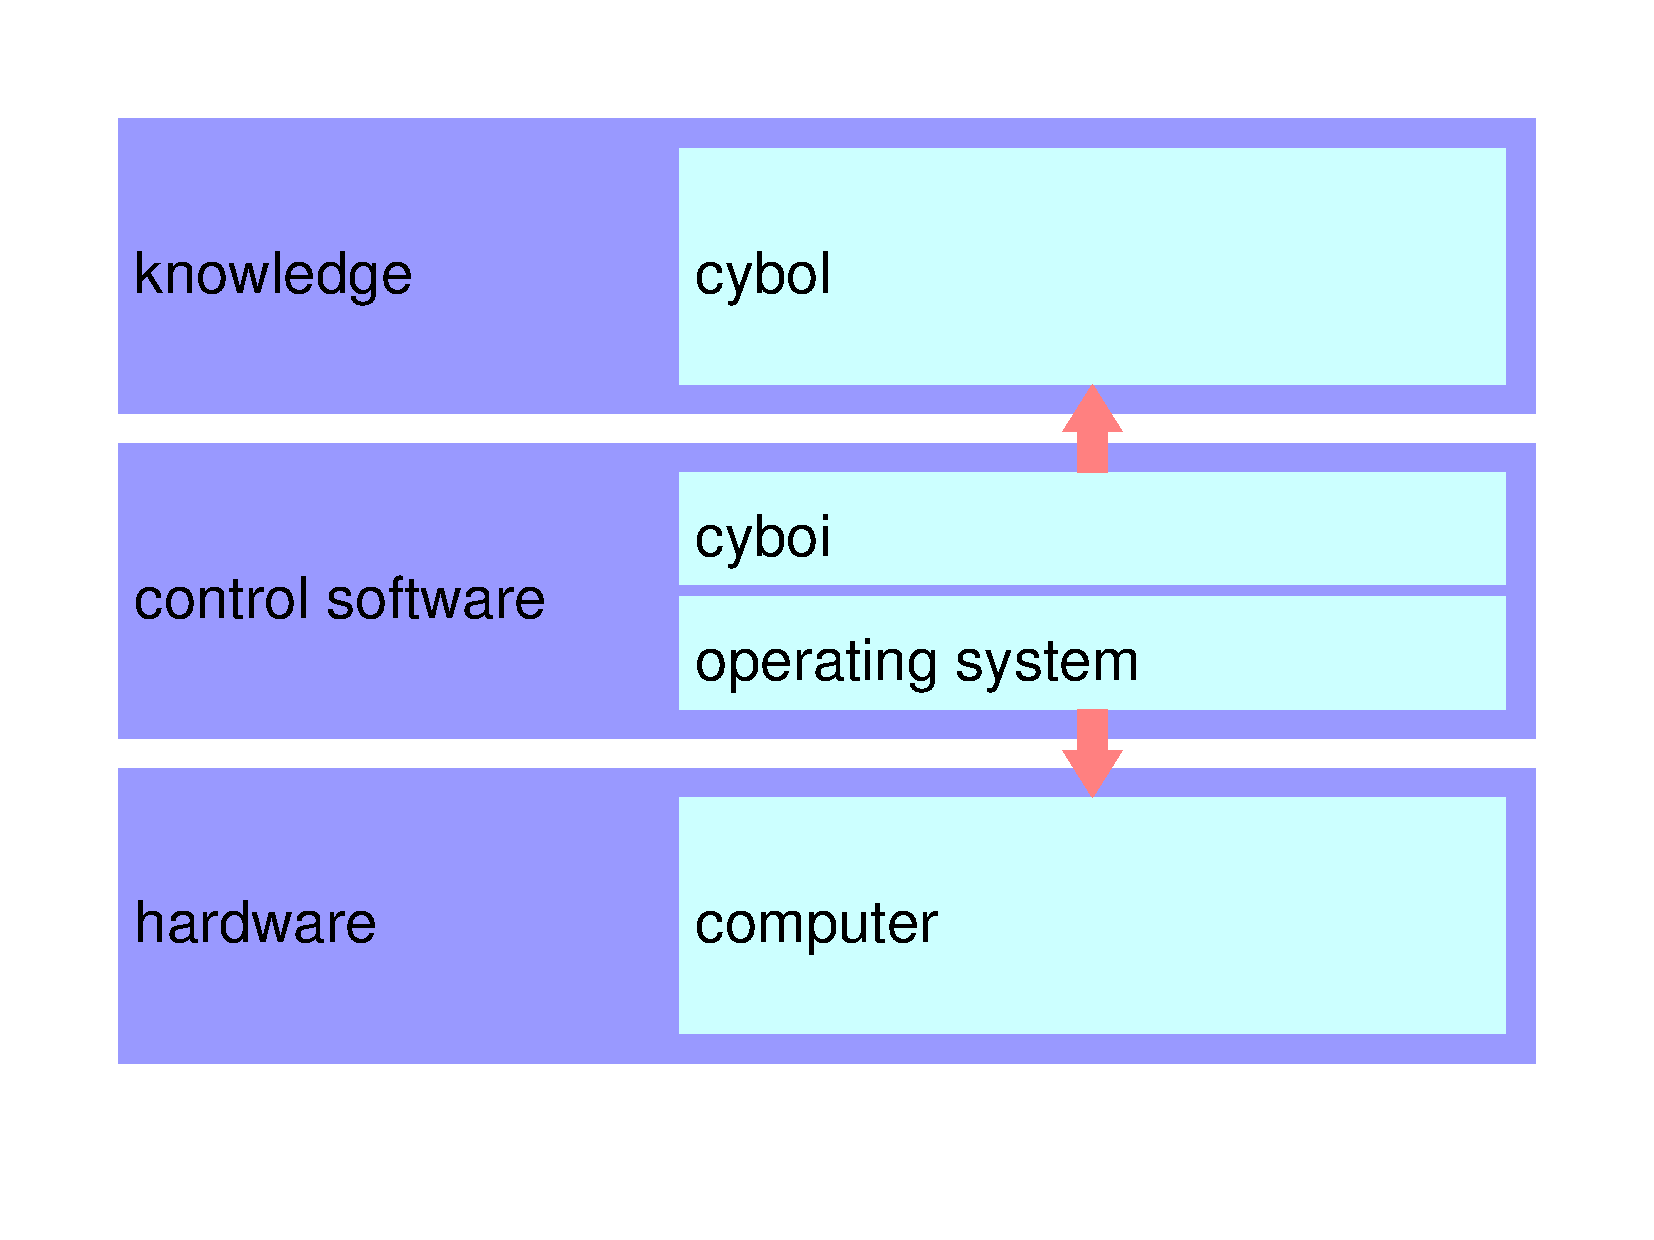
\includegraphics[scale=0.3,angle=-90]{graphic/connection.pdf}
        \caption{Knowledge -- Hardware Connection}
        \label{connection_figure}
    \end{center}
\end{figure}

Three main layers of information crystallise out: \emph{Knowledge},
\emph{Control Software} and \emph{Hardware} (figure \ref{connection_figure}).
Tanenbaum \cite{tanenbaum1999} calls the latter two \textit{logically equivalent}
(section \ref{paradigm_and_language_heading}), because one could replace the
other. It is indeed up to the computer designer to decide how much control
software should get burned into hardware. Hence, the important separation is
between \emph{Knowledge} on one side and \emph{Hardware} together with
\emph{Control Software} on the other.

The previous sections \ref{mind_and_body_heading}, \ref{brain_regions_heading}
and \ref{cell_division_heading} tried to justify this separation by looking at
nature. Knowledge is the equivalent of: \emph{Mind} (philosophically) and the
virtual information stored in a human brain's \emph{Hippocampus} and
\emph{Cerebral Cortex}, as well as of the information encoded in a biological
cell's \emph{Desoxy Ribo Nucleic Acid} (DNA). Hardware and control software are
the equivalent of: (philosophically) \emph{Body}, (neurologically) parts of the
human brain (\emph{Midbrain}, \emph{Basal Ganglia}) which coordinate the input/
output (i/o) of knowledge and (biologically) \emph{Ribo Nucleic Acid} (RNA)
molecules transmitting the genetic information from the DNA into proteins.

Chapters \ref{cybernetics_oriented_language_heading} and
\ref{cybernetics_oriented_interpreter_heading} will describe the
\emph{Cybernetics Oriented Language} (CYBOL) as knowledge specification format
and the \emph{Cybernetics Oriented Interpreter} (CYBOI) as system being able to
handle such knowledge, as well as to serve as hardware interface. All
hardware-controlling functionality needs to be present within either CYBOI or
the underlying \emph{Operating System} (OS) closely coupled with it. Together,
they are the active entity allowing virtual and real world (knowledge and
hardware) to communicate.

The remaining sections of this chapter describe important elements belonging to
a control software's architecture. More detailed descriptions of the
architecture and functionality will be given in chapter
\ref{cybernetics_oriented_interpreter_heading} devoted to CYBOI only.

%
% $RCSfile: memory.tex,v $
%
% Copyright (C) 2002-2008. Christian Heller.
%
% Permission is granted to copy, distribute and/or modify this document
% under the terms of the GNU Free Documentation License, Version 1.1 or
% any later version published by the Free Software Foundation; with no
% Invariant Sections, with no Front-Cover Texts and with no Back-Cover
% Texts. A copy of the license is included in the section entitled
% "GNU Free Documentation License".
%
% http://www.cybop.net
% - Cybernetics Oriented Programming -
%
% http://www.resmedicinae.org
% - Information in Medicine -
%
% Version: $Revision: 1.1 $ $Date: 2008-08-19 20:41:07 $ $Author: christian $
% Authors: Christian Heller <christian.heller@tuxtax.de>
%

\subsection{Memory}
\label{memory_heading}
\index{Memory}
\index{Persistent Memory}
\index{Transient Memory}
\index{Volatile Memory}
\index{Sensory Memory}
\index{Long Term Memory}
\index{LTM}
\index{Short Term Memory}
\index{STM}
\index{Knowledge Memory}
\index{Signal Memory}
\index{Internal Memory}
\index{Input/ Output Memory}
\index{Event Queue}

The application/ domain knowledge a control software processes resides in a
\emph{Memory}. Two different kinds known from \emph{Informatics} are the
\emph{persistent} and \emph{transient} (\emph{volatile}) memory (section
\ref{persistent_and_transient_heading}). For the system architecture
investigated in this section, the term \emph{Memory} does not refer to
hardware, but to a special data structure for knowledge storage.

Section \ref{short_and_long_term_memory_heading} introduced the
\emph{Sensory Memory}, \emph{Long Term Memory} (LTM) and \emph{Short Term Memory}
(STM), so labelled by the science of psychology. Sensory memory stores data
arriving from input organs; LTM stores past contents; STM holds temporary
information to be processed within the system. A knowledge-processing system
with human archetype -- such as the one proposed in this work -- needs to have
equivalents for all three of them. Figure \ref{system_figure} illustrates a
system based on four kinds of memory:

\begin{itemize}
    \item[-] Knowledge Memory (equivalent of LTM)
    \item[-] Signal Memory (equivalent of STM)
    \item[-] Internal Memory (program-internal data)
    \item[-] Input/ Output Memories (sensory data)
\end{itemize}

The \emph{Knowledge Memory} is represented by one single root node that is able
to keep knowledge hierarchies of arbitrary size. The \emph{Signal Memory} is
much the same as the \emph{Event Queue} in classical systems.
\emph{Internal Memory} and \emph{Input/ Output Memories} are helper memories
for storing system-internal parameters.

\begin{figure}[ht]
    \begin{center}
        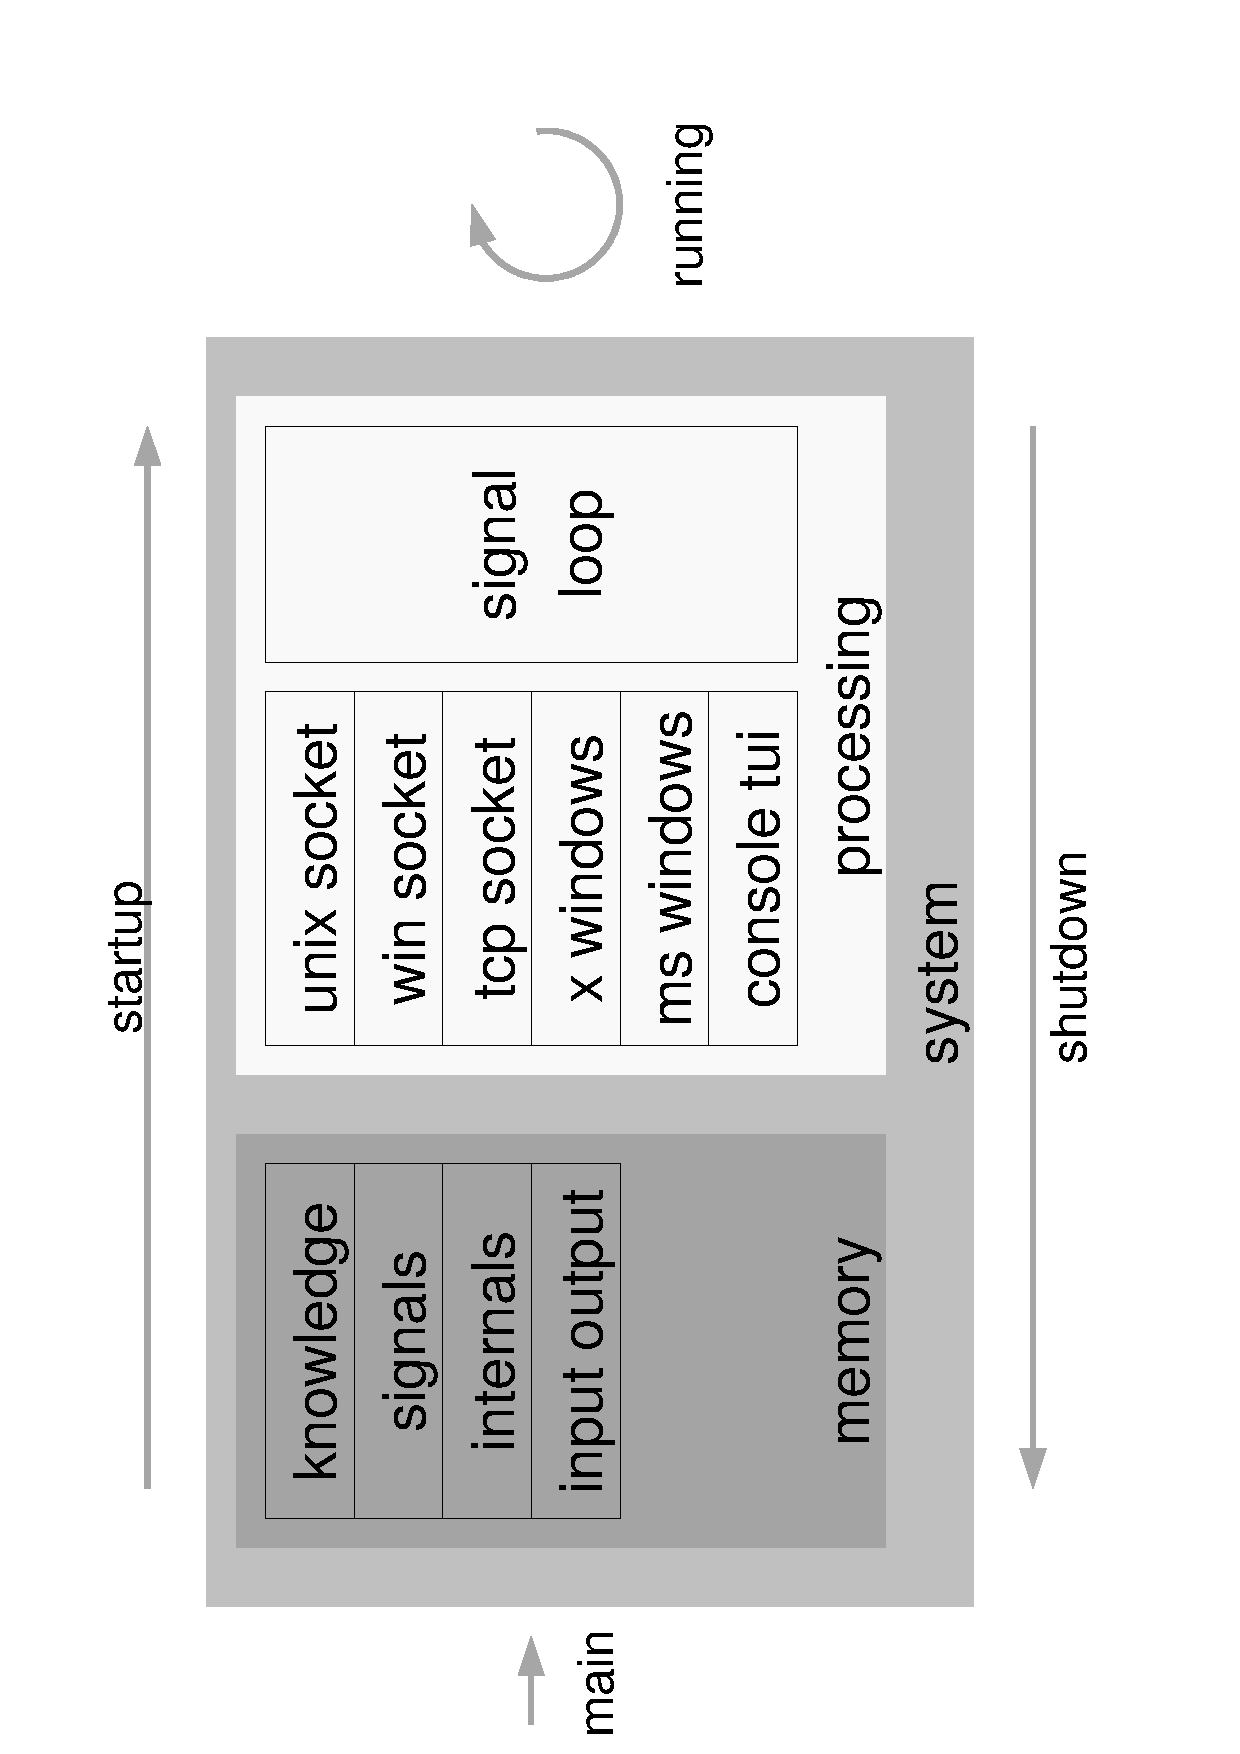
\includegraphics[scale=0.3,angle=-90]{graphic/system.pdf}
        \caption{System with Memory Structures, Processing Loops and Lifecycle}
        \label{system_figure}
    \end{center}
\end{figure}

%
% $RCSfile: processing.tex,v $
%
% Copyright (C) 2002-2008. Christian Heller.
%
% Permission is granted to copy, distribute and/or modify this document
% under the terms of the GNU Free Documentation License, Version 1.1 or
% any later version published by the Free Software Foundation; with no
% Invariant Sections, with no Front-Cover Texts and with no Back-Cover
% Texts. A copy of the license is included in the section entitled
% "GNU Free Documentation License".
%
% http://www.cybop.net
% - Cybernetics Oriented Programming -
%
% http://www.resmedicinae.org
% - Information in Medicine -
%
% Version: $Revision: 1.1 $ $Date: 2008-08-19 20:41:08 $ $Author: christian $
% Authors: Christian Heller <christian.heller@tuxtax.de>
%

\subsection{Processing}
\label{processing_heading}
\index{Processing of Knowledge}
\index{Signal}
\index{Event}
\index{Signal Memory}
\index{Event Queue}
\index{Signal Loop}
\index{Waiting Loop}
\index{Priority of a Signal}
\index{Prioritising}
\index{Operating System}
\index{OS}
\index{Intra System Communication}
\index{Inter System Communication}
\index{Message}

While knowledge as such is static at a given time instant, its \emph{Processing}
and manipulation over time are dynamic. The processing is triggered by some
\emph{Signal} (also called \emph{Event}), which is a state change known to the
system. Such \textit{signs with defined meaning}, as the Duden Encyclopedia
\cite{duden} calls them, can be most different in their appearance and
communication channel used.

Signals are commonly stored in a \emph{Signal Memory} (also called
\emph{Event Queue}), as mentioned in the previous section. An endlessly running
\emph{Signal Loop} (also called \emph{Waiting Loop}) as illustrated in figure
\ref{system_figure} is constantly checking the signal memory for new signals.
Once a signal is detected, it gets removed from the signal memory and handled
by the system. The signal with highest \emph{Priority} is processed first. The
later chapter \ref{cybernetics_oriented_interpreter_heading} will explain
further details and deliver a more functional illustration (figure
\ref{dependencies_figure}).

Section \ref{brain_regions_heading} mentioned the \emph{Hypothalamus} and
\emph{Limbic System} as parts of the human brain producing emotions. Section
\ref{information_processing_model_heading} wrote that the processing of a signal
may be greatly influenced by the meaningfulness or \emph{Emotional Content} of
an item. Well, software systems do not work with emotions, but signals can be
assigned a \emph{Priority}, which is somewhat comparable. \emph{Prioritising}
as technique stems from \emph{Operating System} (OS) research and can be well
applied in the described knowledge-processing system: Signals can be filtered
in a way that unimportant signals get discarded; urgent signals get processed
right away; less important but meaningful signals get queued for later handling.

All \emph{intra-system} and \emph{inter-system} communication is based on the
exchange of knowledge via signals. A signal can transport simple or more complex
\emph{Messages}, mostly in encoded form. The communication details, including
encoding and decoding procedures for knowledge model translation, and the logic
after which an input state gets transferred into an output state are the topic
of chapter \ref{state_and_logic_heading}.

Besides the \emph{declarative} \emph{Long Term Memory} (LTM), section
\ref{short_and_long_term_memory_heading} mentioned the \emph{procedural}
(non-declarative) LTM, enabling humans to carry out a \emph{Background Task},
without having to consciously control it. A similar principle is applied for
input/ output (i/o) handling, in the described knowledge processing system.
Independent \emph{Threads} running their own loops control a special i/o
mechanism (like \emph{UNIX socket etc.}), each (figure \ref{system_figure}).

\section{An Extended Component Lifecycle}

The CYBOP lifecycle of components is an extension of the lifecycle idea of Apache
-- basically the same idea but another background and realization.\\
All \emph{whole-part associations} between objects were organized
under the rules of the component lifecycle. Analogous to the
lifecycle of organic cells, the relations were created and
destroyed in a sequence of lifecycle steps. These steps are
realized as method calls on the components (see figure \ref{State
Diagram of CYBOB's Component Lifecycle}).
\includepicture{8}{eps/lebenszyklusEng.eps}{State Diagram of CYBOB's Component Lifecycle}{State Diagram of CYBOB's Component Lifecycle}{State Diagram of CYBOB's Component Lifecycle} {State Diagram of CYBOB's Component Lifecycle}

%\input{instantiation} (clone, serialisation, knowledge template and -instance)
%\input{template_and_model} (activate when replication/ cloning is activated, too
% = persistent knowledge template versus transient knowledge model

